% mnras_template.tex 
%
% LaTeX template for creating an MNRAS paper
%
% v3.0 released 14 May 2015
% (version numbers match those of mnras.cls)
%
% Copyright (C) Royal Astronomical Society 2015
% Authors:
% Keith T. Smith (Royal Astronomical Society)

% Change log
%
% v3.0 May 2015
%    Renamed to match the new package name
%    Version number matches mnras.cls
%    A few minor tweaks to wording
% v1.0 September 2013
%    Beta testing only - never publicly released
%    First version: a simple (ish) template for creating an MNRAS paper

%%%%%%%%%%%%%%%%%%%%%%%%%%%%%%%%%%%%%%%%%%%%%%%%%%
% Basic setup. Most papers should leave these options alone.
\documentclass[fleqn,usenatbib]{mnras}

% MNRAS is set in Times font. If you don't have this installed (most LaTeX
% installations will be fine) or prefer the old Computer Modern fonts, comment
% out the following line
\usepackage{newtxtext,newtxmath}
% Depending on your LaTeX fonts installation, you might get better results with one of these:
%\usepackage{mathptmx}
%\usepackage{txfonts}

% Use vector fonts, so it zooms properly in on-screen viewing software
% Don't change these lines unless you know what you are doing
\usepackage[T1]{fontenc}
\usepackage{ae,aecompl}


%%%%% AUTHORS - PLACE YOUR OWN PACKAGES HERE %%%%%

% Only include extra packages if you really need them. Common packages are:
\usepackage{graphicx}	% Including figure files
\usepackage{amsmath}	% Advanced maths commands
\usepackage{amssymb}	% Extra maths symbols


%%%%%%%%%%%%%%%%%%%%%%%%%%%%%%%%%%%%%%%%%%%%%%%%%%

%%%%% AUTHORS - PLACE YOUR OWN COMMANDS HERE %%%%%
\newcommand{\beqa}{\begin{eqnarray}} 
\newcommand{\cmark}{\ding{51}}%
\newcommand{\xmark}{\ding{55}}%
\newcommand{\eeqa}{\end{eqnarray}}
\newcommand{\Abst}[1]{\;#1}
\newcommand{\bsub}{\begin{subequations}}
\newcommand{\esub}{\end{subequations}}
\newcommand{\beal}{\begin{align}}
\newcommand{\ealn}{\end{align}}
\newcommand{\lm}{$L_{max}$~}
\newcommand{\tb}{$t_B$(max)\,}
\newcommand{\Mni}{$\rm M_{^{56}Ni}$~}
\newcommand{\Ms}{M$_{\sun}$}
\newcommand{\ejm}{M$_{ej}$\,}
\newcommand{\dm}{$\Delta m_{15}(B)$\,}
\newcommand{\mc}{$\rm M_{Ch}$\,}
\newcommand{\Nif}{$\rm ^{56}Ni$\,} 
\newcommand{\Cif}{$\rm ^{56}Co$\,}
\newcommand{\Fif}{$\rm ^{56}Fe$}
\newcommand{\ksm}{${\rm km~s^{-1}~Mpc^{-1}}$}
\newcommand{\s}{\rm M$_{\sun}$}
\newcommand{\sbv}{$s_{BV}$\,}
\newcommand{\egs}{$\cdot$ 10$^{43}$ erg s$^{-1}$}
\newcommand{\kms}{$\mathrm{km\;s^{-1}}$}
\newcommand{\kmpc}{$\mathrm{km\; s^{-1}\; Mpc^{-1}}$}
\newcommand{\ho}{$H_0$\,}
\newcommand{\sigint}{$\sigma_{\rm int}$}
\newcommand{\sigcz}{$\sigma_{cz}$\,}
\newcommand{\avg}[1]{\left\langle{#1}\right\rangle}
% Please keep new commands to a minimum, and use \newcommand not \def to avoid
% overwriting existing commands. Example:
%\newcommand{\pcm}{\,cm$^{-2}$}	% per cm-squared

%%%%%%%%%%%%%%%%%%%%%%%%%%%%%%%%%%%%%%%%%%%%%%%%%%

%%%%%%%%%%%%%%%%%%% TITLE PAGE %%%%%%%%%%%%%%%%%%%

% Title of the paper, and the short title which is used in the headers.
% Keep the title short and informative.
% \title[$\ion{Ni}{II}$ in nebular spectra of SN\,Ia]{Evidence for consistent shifts of singly and doubly ionized iron group material from SN\,Ia nebular spectroscopy}
\title[Nickel and iron in SNe Ia]{%The evolution of temperature and density in the iron rich ejecta of Type Ia supernovae reveals a wide range of neutron-rich material masses 
Sub-Chandrasekhar progenitors favoured for type Ia supernovae: Evidence from late-time spectroscopy.
}
% The list of authors, and the short list which is used in the headers.
% If you need two or more lines of authors, add an extra line using \newauthor
\author[A. Fl\"ors et al.]{
A. Fl\"ors,$^{1,2,3}$\thanks{E-mail: afloers@mpa-garching.mpg.de}
J. Spyromilio,$^{1}$
S. Taubenberger,$^{2}$
R. Cartier,$^{4}$
S. Blondin,$^{5,6}$
\newauthor
B. Leibundgut,$^{1}$
L. Dessart,$^{6}$
S. Dhawan,$^{7}$
W. Hillebrandt$^{2}$
\\
% List of institutions
$^{1}$European Southern Observatory, Karl-Schwarzschild-Stra\ss e 2,
D-85748 Garching bei M\"unchen, Germany\\
$^{2}$Max-Planck-Institut f\"ur Astrophysik, Karl-Schwarzschild-Stra\ss e 1, D-85748 Garching bei M\"unchen, Germany\\
$^{3}$Physik-Department, Technische Universit\"at M\"unchen, James-Franck-Stra\ss e 1, D-85748 Garching bei M\"unchen, Germany\\
$^{4}$Cerro Tololo Inter-American Observatory, National Optical Astronomy Observatory, Casilla 603, La Serena, Chile\\
$^{5}$Aix Marseille Univ, CNRS, LAM, Laboratoire d’Astrophysique de Marseille, Marseille, France\\
$^{6}$Unidad Mixta Internacional Franco-Chilena de Astronom\'ia, CNRS/INSU UMI 3386, \\
$^{\,\,\,}$and Departamento de Astronom\'ia, Universidad de Chile, Camino El Observatorio 1515,Las Condes, Santiago, Chile\\
$^{7}$The Oskar Klein Centre, Physics Department, Stockholm University, Albanova University Center, SE 106 91 Stockholm, Sweden
}

% These dates will be filled out by the publisher
\date{Accepted XXX. Received YYY; in original form ZZZ}

% Enter the current year, for the copyright statements etc.
\pubyear{2019}

% Don't change these lines
\begin{document}
\label{firstpage}
\pagerange{\pageref{firstpage}--\pageref{lastpage}}
\maketitle

% Abstract of the paper
\begin{abstract}
A non-local-thermodynamic-equilibrium (NLTE) level population model of the first and second ionisation stages of iron, nickel and cobalt is used to fit a sample of XShooter optical + near-infrared (NIR) spectra of Type Ia supernovae (SNe Ia). From the ratio of the NIR lines to the optical lines limits can be placed on the temperature and density of the emission region. We find a similar evolution of these parameters across our sample. Using the evolution of the \ion{Fe}{II} 12570\AA\,to 7155\,\AA\,line as a prior in fits of spectra covering only the optical wavelengths we show that the 7200\,\AA\,feature is fully explained by [\ion{Fe}{II}] and [\ion{Ni}{II}] alone. This approach allows us to determine the abundance of \ion{Ni}{II}/\ion{Fe}{II} for a large sample of 150 optical spectra with uncertainties small enough to distinguish between Chandrasekhar mass (M$_{\text{Ch}}$) and sub-Chandrasekhar mass (sub-M$_{\text{Ch}}$) explosion models. We conclude that the majority (85\%) of normal SNe Ia have a Ni/Fe abundance that is in agreement with predictions of sub-M$_{\text{Ch}}$ explosion simulations of $\sim Z_\odot$ progenitors. Only a small fraction (9\%) of objects in the sample have a Ni/Fe abundance in agreement with M$_{\text{Ch}}$ explosion models.
\end{abstract}

% Select between one and six entries from the list of approved keywords.
% Don't make up new ones.
\begin{keywords}
keyword1 -- keyword2 -- keyword3
\end{keywords}

%%%%%%%%%%%%%%%%%%%%%%%%%%%%%%%%%%%%%%%%%%%%%%%%%%

%%%%%%%%%%%%%%%%% BODY OF PAPER %%%%%%%%%%%%%%%%%%

\section{Introduction}
Type Ia supernovae (SNe Ia) are a remarkably homogeneous class of transients which, it is postulated, originate from the explosion of a white dwarf (WD) star in a binary system. Radioactive \ensuremath{^{56}{\rm Ni}} produced in the thermonuclear explosion of the electron-degenerate matter \citep{1960ApJ...132..565H} powers the light curve \citep{1969ApJ...157..623C, 1994ApJ...426L..89K} for several years. Even though SNe Ia have been used as distance indicators for several decades and significantly contributed to our current understanding of cosmology \citep[$\Lambda$CDM and the accelerated expansion of the universe, ][]{1998AJ....116.1009R, 1999ApJ...517..565P}, the precise mechanism that leads to the thermonuclear runaway reaction and the progenitor system remains elusive. 

Two channels that can lead to the explosion of a WD as a SNe Ia have been extensively discussed in the literature. In M$_{\text{Ch}}$ explosions the flame propagates either as a deflagration \citep{2014MNRAS.438.1762F} or a delayed detonation \citep{2013MNRAS.429.1156S}. The explosion is naturally triggered by an increase of the central temperature as the WD accretes material from its companion and comes close to the Chandrasekhar mass limit ($M\simeq\,$M$_{\text{Ch}}$). In the sub-M$_{\text{Ch}}$ channel the central temperature of the primary white dwarf never reaches conditions that are sufficient to ignite carbon. However, an explosion significantly below the M$_{\text{Ch}}$ may be triggered through dynamical processes such as mergers \citep{2010Natur.463...61P}, double detonations \citep{2010A&A...514A..53F, 2018ApJ...854...52S} or head-on collisions \citep{2013ApJ...778L..37K}. For such systems the flame propagates as a pure detonation \citep{2010ApJ...714L..52S}.

The search for solutions to the SN Ia progenitor problem has been the focus of many studies. 
For historical supernova remnants one can search for a surviving companion star which was ejected at velocities of a few hundred km\,s$^{-1}$, though no promising candidates have been found so far (\citeauthor{2018MNRAS.479..192K} \citeyear{2018MNRAS.479..192K} for SN\,1006, \citeauthor{2018MNRAS.479.5696K} \citeyear{2018MNRAS.479.5696K} for SN\,1572). 
Non-degenerate donor stars of SNe Ia in nearby galaxies should also be visible in deep images as their brightness increases by a factor of $\sim10 - 10^3$, though again, no donor stars have been found for a sample of the closest SNe Ia in recent times \citep{2013ApJ...765..150S}. 

The growth of a white dwarf star to the M$_{\text{Ch}}$ limit requires a steady transfer of material from the companion. Material which was expelled from the companion but not accreted on the white dwarf enriches the circumstellar material (CSM). When the blast wave from the SN explosion runs through the CSM, electrons are accelerated to relativistic speeds and produce radio emission through synchrotron radiation \citep{1982ApJ...259..302C, 1998ApJ...499..810C, 2006ApJ...651..381C}. For a nearby SN Ia such as SN\,2011fe radio emission should be observable if it exploded in the single degenerate channel. However, no radio emission was found by \citet{2012ApJ...746...21H} for SN\,2011fe . 

One can also distinguish the two channels from direct observations of the aftermath of the explosion itself. Unfortunately, the uniformity of explosion model predictions of SNe Ia makes this a challenging task. A promising difference between M$_{\text{Ch}}$ and sub-M$_{\text{Ch}}$ models is the mass fraction of neutronized species produced in the explosion. While the progenitor metallicity affects how much neutron-rich material can be produced in both channels, additional neutrons are only available for explosions close to the M$_{\text{Ch}}$ due to the high central densities ($\rho_{\text{cen}} \sim 2\times 10^9$\,g\,cm$^{-3}$) which allow electron capture reactions to take place \citep{1999ApJS..125..439I, 2013MNRAS.429.1156S}. 

X-ray spectroscopy of SN remnants in the Milky Way (MW) and the Large and Small Magellanic Clouds (LMC \& SMC) allowed \citet{2013ApJ...767L..10P}, \citet{2014HEAD...1430402Y}, \citet{2015ApJ...801L..31Y}, \citet{2017ApJ...843...35M} and \citet{2019arXiv190605972S} to estimate the fraction of the neutron-rich stable iron-peak isotopes $^{55}$Mn and $^{58}$Ni. They find considerable differences across their sample, but the number of objects for which such a study can be done is quite limited. 

Contributions of slowly-decaying neutron-rich material
{\bf JSP: 
(e.g. $^{57}$Co the daughter product of $^{57}$Ni) 
}
%($^{57}$Co from the decayed $^{57}$Ni) 
to the quasi-bolometric light curve of the nearby SN\,2011fe at >1000\,days after the explosion were investigated by \citet{2017hst..prop15192S}, \citet{2017MNRAS.468.3798D} and \citet{2017MNRAS.472.2534K}. This method was used for other nearby transients SN\,2012cg \citep{2016ApJ...819...31G}, SN\,2013aa \citep{2018ApJ...857...88J}, SN\,2014J \citep{2018ApJ...852...89Y}, SN\,2014lp \citep{2018ApJ...866...10G} and SN\,2015F \citep{2018ApJ...859...79G}. However, the physical processes relevant at such late phases have long time constants and their onset is poorly constrained by the data \citep{2015ApJ...814L...2F}. In particular, it remains unclear what fraction of the radioactive decay energy is converted into optical photons as the majority of the energy is expected to come out in the mid-IR. 

SNe Ia complete their transition into the nebular phase roughly half a year after the explosion when the ejecta become fully transparent and the bare iron core which gives insight into the explosion physics is visible. Nebular phase spectral models build on the early work of \citet{1980PhDT.........1A} and many  authors over the years \citep{1992MNRAS.258P..53S, 1992ApJ...390..602K, 1994ApJ...426L..89K, 2005A&A...437..983K, 2007Sci...315..825M, 2015ApJ...814L...2F, 2017ApJ...845..176B, 2018MNRAS.477.3567M, 2018ApJ...861..119D} with spectral synthesis codes of varying complexity.

The method presented herein enables the use optical lines of Ni and Fe to constrain the fraction of neutron rich material in the ejecta. This approach increases the number of objects for which the analysis can be performed by about one order of magnitude compared to the number of optical+NIR spectra currently available. The analysis is made possible by using a small sample of optical+NIR spectra to determine the relative strength of the NIR to the optical emission of \ion{Fe}{II}. With this relation we can model archival optical nebular spectra which do not have NIR observations. From the fits of the model to observed spectra we determine the Ni to Fe ratio. We estimate the systematic uncertainty of the method and show that emission lines from singly ionized iron and nickel are sufficient to model the 7200\,\AA\,feature. Finally, we discuss the implications of the determined Ni to Fe ratio of the large sample of more than 100 spectra on the various explosion model predictions.
\section{Observations}
\label{SectionObservations}
We extend the XShooter sample of nearby SNe Ia in the nebular phase from \citet{2018MNRAS.477.3567M} with SN\,2015F (PI M. Sullivan, program IDs 095.A-0316, 096.D-0829, 097.D-0967 and 098.D-0692) and SN\,2017bzc (PI L. Dessart, program ID 0100.D-0285). The epochs of the additional spectra range from $\sim$\,200 days to $\sim$\,420 days after the explosion. An overview of the observations is given in Table \ref{tab:Observations}.

XShooter is an echelle spectrograph with three arms (UVB, VIS and NIR) covering the wavelength range of $\sim$\,3000--25000\,\AA\,located at the Very Large Telescope (VLT). The resolution of the individual arms depends on the slit widths used. For the observations presented in this work slit widths of 1.0 (UVB), 0.9 (VIS) and 0.9 (NIR) arcseconds have been used. The corresponding resolution of the three arms is therefore 5400, 8900 and 5600, respectively. The spectra were reduced using the ESO pipeline with the XShooter module, producing flux-calibrated one-dimensional spectra in each of the three arms \citep{2010SPIE.7737E..28M,2013A&A...559A..96F}. We also used a custom postprocessing pipeline to combine the rectified 2D-images, perform the sky-subtraction and extract the spectrum (\url{https://github.com/jselsing/xsh-postproc}).


\begin{table*}
	\caption{Overview of the observations}
	\label{tab:Observations}
    \begin{tabular}{lcclccccc}
    	\hline 
    	SN name   & Observation & Observation & Phase$^a$     & E($B-V$)$^b$ & Helio. z$^c$ & Host galaxy & Exposure \\
                  & MJD         & date        &  & (mag)    &          &             & time (s) \\
		\hline                   
    % 	SN\,2012ht  &             & +433d &             \\
    % 	SN\,2013aa  &             & +360d &             \\
    % 	          &             & +425d &             \\
    %     SN\,2012fr  &             & +357d &             \\
    %     SN\,2012cg  &             & +339d &             \\
    %     SN\,2013cs  &             & +303d &             \\
    %     SN\,2013ct  &             & +229d &             \\
        
    %     PSNJ1149  &             & +206d &             \\
        SN\,2015F   & 57287.4     & 2015 Sept 22& +181d & 0.260$\pm$0.021$^d$ & 0.00489 & NGC 2442 & 720\\
                  & 57331.4     & 2015 Nov 05 & +225d &                     & & & 1200\\
                  & 57345.3     & 2015 Nov 19 & +239d &                     & & & 3600\\
                  & 57372.2     & 2015 Dec 16 & +266d &                     & & & 7600\\
                  & 57512.0     & 2016 May 04 & +406d &                     & & & 3800\\
        SN\,2017bzc & 58039.5     & 2017 Oct 12 & +215d & 0.0122$\pm$0.0002   & 0.00536 & NGC 7552 & 10080\\
		\hline
			\end{tabular}
		\begin{flushleft}
         $^a$Phase of late-time spectrum calculated with respect to maximum light. \\
         $^b$Galactic $E$(\textit{B-V}) values from \protect \cite{2011ApJ...737..103S}.\\
         $^c$Heliocentric redshifts are from the Nasa Extragalactic Database (NED).\\
         $^d$Additional host galaxy extinction of $E$(\textit{B-V})=0.085 mag was found for SN 2015F by \citet{2017MNRAS.464.4476C}. The value given in the table is the combined MW and host galaxy $E$(\textit{B-V}). \\
 \end{flushleft}
 \end{table*}

Nebular phase spectra of SNe Ia exhibit a number of broad ($\approx7\,000$ to $9\,000$ km\,s$^{-1}$) emission features. In the NIR, we identify the strongest features as emission by singly ionized [\ion{Fe}{II}] and [\ion{Co}{II}]. The 1.090\,$\mu$m (a$^3$F$_4$--b$^3$F$_4$) transition of [\ion{Co}{II}] is evident in the data and decreases in strength according to the decay of $^{56}$Co to $^{56}$Fe \citep{2004A&A...426..547S, 2018A&A...620A.200F}. The emission feature at 1.3\,$\mu$m is identified as the 1.257\,$\mu$m a$^6$D--a$^4$D multiplet of [\ion{Fe}{II}]. The double peaked feature around 1.6\,$\mu$m is composed of a blend of [\ion{Fe}{II}] and [\ion{Co}{II}] lines of the multiplets a$^4$F--a$^4$D and a$^5$F--b$^3$F, respectively. Bluewards of the strong telluric absorption feature at $\sim$ 1.85\,$\mu$m we also detect the a$^{2}$F$_{7/2}$--a$^{4}$F$_{9/2}$ line of [\ion{Ni}{II}] in spectra with high SNR \citep{2018A&A...619A.102D}.

In the optical we see blends of singly and doubly ionized Fe, Co and Ni. The strong feature at 4700\,\AA\,originates mainly from the $3d^6$\,$^5$D--$^3$F multiplet of [\ion{Fe}{III}] \citep{1980PhDT.........1A, 1994ApJ...426L..89K}. The broad emission centered around $5900$\,\AA\, is primarily due to [\ion{Co}{III}] in the a$^4$F--a$^2$G multiplet. The identification of the $5900$\,\AA\, [\ion{Co}{III}] feature is secured by the fact that the relative strength of this feature with respect to e.g. the [\ion{Fe}{III}] $4700$\,\AA\,feature decreases with time as predicted by radioactive decay of $^{56}$Co \citep{1994ApJ...426L..89K, 2015MNRAS.454.3816C}. Near the $7200$\,\AA\,region the spectra exhibit emission lines of the [\ion{Fe}{II}] multiplets a$^4$F--a$^2$G and a$^6$D--a$^4$P and the [\ion{Ni}{II}] multiplet z$^2$D--a$^2$F. The identification of the various emission lines in the optical and NIR of SNe Ia in the nebular phase has been extensively discussed in the literature and is considered secure. A detailed overview of the strongest emission lines is given in Table \ref{tab:LineID}.
\begin{table}
	\centering
	\caption{Selected forbidden lines of singly and doubly ionized Fe, Co and Ni in the optical and NIR} 
	\label{tab:LineID}
    \begin{tabular}{lcc}
    	\hline 
    	$\lambda_{\text{rest}}$($\mu$m) & Ion & Transition\\
		\hline  
		0.4418 & [\ion{Fe}{II}] & a$^6$D$_{9/2}\,-\,$b$^4$F$_{9/2}$\\ 
		0.4659 & [\ion{Fe}{III}] & $^5$D$_{4}\,-\,^3$F$_{4}$\\
		0.4891 & [\ion{Fe}{II}] & a$^6$D$_{7/2}\,-\,$b$^4$P$_{5/2}$\\ 
		0.5160 & [\ion{Fe}{II}] & a$^4$F$_{9/2}\,-\,$a$^4$H$_{13/2}$\\ 
		0.5272 & [\ion{Fe}{III}] & $^5$D$_{3}\,-\,^3$P$_{2}$\\
        0.5528 & [\ion{Fe}{II}] & a$^4$F$_{7/2}\,-\,$a$^2$D$_{5/2}$\\
        0.5888 & [\ion{Co}{III}] & a$^4$F$_{9/2}\,-\,$a$^2$G$_{9/2}$\\
        0.5908 & [\ion{Co}{III}] & a$^4$F$_{7/2}\,-\,$a$^2$G$_{7/2}$\\
        0.6197 & [\ion{Co}{III}] & a$^4$F$_{7/2}\,-\,$a$^2$G$_{9/2}$\\
        0.6578 & [\ion{Co}{III}] & a$^4$F$_{9/2}\,-\,$a$^4$P$_{5/2}$\\
        0.6855 & [\ion{Co}{III}] & a$^4$F$_{7/2}\,-\,$a$^4$P$_{3/2}$\\
        0.7155 & [\ion{Fe}{II}] & a$^4$F$_{9/2}\,-\,$a$^2$G$_{9/2}$\\
        0.7172 & [\ion{Fe}{II}] & a$^4$F$_{7/2}\,-\,$a$^2$G$_{7/2}$\\
        0.7378 & [\ion{Ni}{II}] & z$^2$D$_{5/2}\,-\,$a$^2$F$_{7/2}$\\
		0.7388 & [\ion{Fe}{II}] & a$^4$F$_{5/2}\,-\,$a$^2$G$_{7/2}$\\
        0.7414 & [\ion{Ni}{II}] & z$^2$D$_{3/2}\,-\,$a$^2$F$_{5/2}$\\
        0.7453 & [\ion{Fe}{II}] & a$^4$F$_{7/2}\,-\,$a$^2$G$_{9/2}$\\
        0.7638 & [\ion{Fe}{II}] & a$^6$D$_{7/2}\,-\,$a$^4$P$_{5/2}$\\
        0.7687 & [\ion{Fe}{II}] & a$^6$D$_{5/2}\,-\,$a$^4$P$_{3/2}$\\
        0.8617 & [\ion{Fe}{II}] & a$^4$F$_{9/2}\,-\,$a$^4$P$_{5/2}$\\
        0.9345 & [\ion{Co}{II}] & a$^3$F$_{3}\,-\,$a$^1$D$_{2}$\\
        0.9704 & [\ion{Fe}{III}] & $^3$H$_{6}\,-\,^1$I$_{6}$\\
        1.0190 & [\ion{Co}{II}] & a$^3$F$_{4}\,-\,$b$^3$F$_{4}$\\
        1.0248 & [\ion{Co}{II}] & a$^3$F$_{3}\,-\,$b$^3$F$_{3}$\\
        1.0611 & [\ion{Fe}{III}] & $^3$F$_{4}\,-\,^1$G$_{4}$\\
        1.2570 & [\ion{Fe}{II}] & a$^6$D$_{9/2}\,-\,$a$^4$D$_{7/2}$\\
        1.2943 & [\ion{Fe}{II}] & a$^6$D$_{5/2}\,-\,$a$^4$D$_{5/2}$\\
        1.3206 & [\ion{Fe}{II}] & a$^6$D$_{7/2}\,-\,$a$^4$D$_{7/2}$\\
        1.5335 & [\ion{Fe}{II}] & a$^4$F$_{9/2}\,-\,$a$^4$D$_{5/2}$\\
        1.5474 & [\ion{Co}{II}] & a$^5$F$_{5}\,-\,$b$^3$F$_{4}$\\
        1.5488 & [\ion{Co}{III}] & a$^2$G$_{9/2}\,-\,$a$^2$H$_{9/2}$\\
        1.5995 & [\ion{Fe}{II}] & a$^4$F$_{7/2}\,-\,$a$^4$D$_{3/2}$\\
        1.6440 & [\ion{Fe}{II}] & a$^4$F$_{9/2}\,-\,$a$^4$D$_{7/2}$\\
        1.7416 & [\ion{Co}{III}] & a$^2$G$_{9/2}\,-\,$a$^2$H$_{11/2}$\\ 
        1.74548 & [\ion{Fe}{II}] & a$^4$F$_{3/2}\,-\,$a$^4$D$_{1/2}$\\ 
        1.8098 & [\ion{Fe}{II}] & a$^4$F$_{7/2}\,-\,$a$^4$D$_{7/2}$\\ 
        1.9390 & [\ion{Ni}{II}] & a$^2$F$_{7/2}\,-\,$a$^4$F$_{9/2}$\\
        2.0028 & [\ion{Co}{III}] & a$^4$P$_{5/2}\,-\,$a$^2$P$_{3/2}$\\ 
        2.0157 & [\ion{Fe}{II}] & a$^2$G$_{9/2}\,-\,$a$^2$H$_{9/2}$\\ 
        2.2184 & [\ion{Fe}{III}] & $^3$H$_{6}\,-\,^3$G$_{5}$\\
		\hline
	\end{tabular}
\end{table}

 
 \begin{figure*}
    \centering
    \begin{minipage}{.475\textwidth}
        \centering
        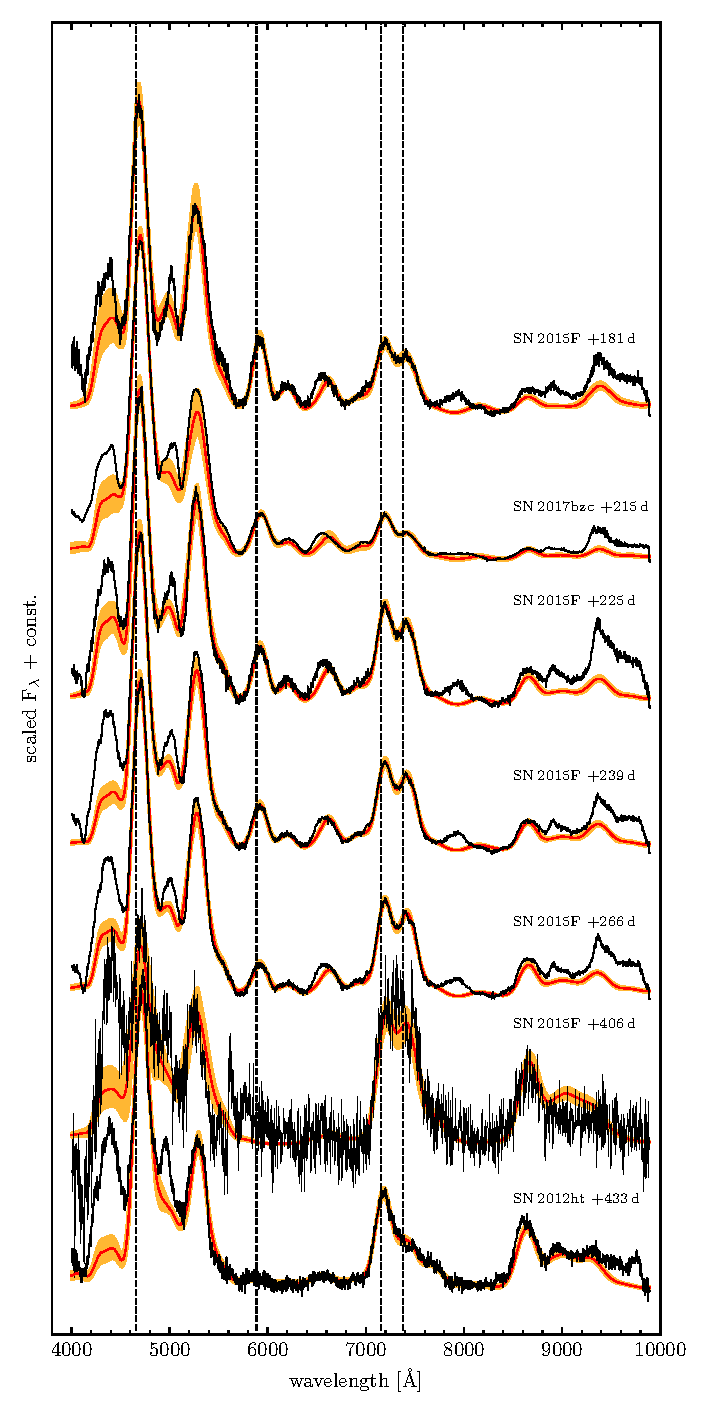
\includegraphics[width=1\linewidth]{plots/Spectra_15F_XSHOOTER_VIS.pdf}
    \end{minipage}%
    \begin{minipage}{.475\textwidth}
        \centering
        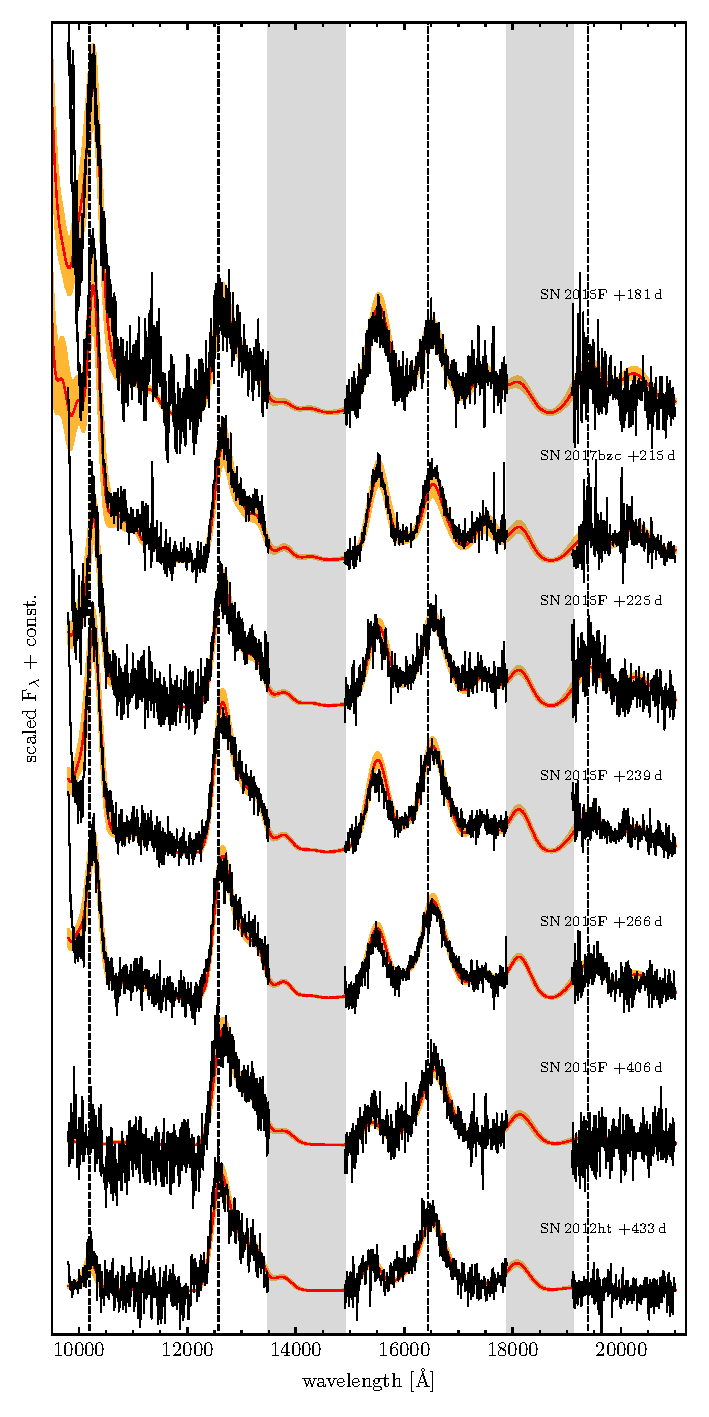
\includegraphics[width=1\linewidth]{plots/Spectra_15F_XSHOOTER_NIR.pdf}
    \end{minipage}
    \caption{Optical (left) and NIR (right) spectra of SN\,2015F and SN\,2017bzc obtained with XShooter at the VLT. We also show the spectrum and the corresponding fit to SN\,2012ht presented in \citep{2018MNRAS.477.3567M}. The spectra are arranged in epoch starting with the youngest at the top. The spectra have been corrected for telluric absorption but not for extinction and host galaxy redshift. Instead, we redshift and extinguish the spectral models. Fluxes are normalized to the $4\,700\,$\AA\,[\ion{Fe}{III}] feature (optical) and $12\,600\,$\AA\,[\ion{Fe}{II}] feature (NIR). In the NIR the bands of heavy telluric absorption are masked in grey. In the optical the rest wavelengths of the 4659\,\AA\,[\ion{Fe}{III}], the 5888\,\AA\,[\ion{Co}{III}], the 7155\,\AA\,[\ion{Fe}{II}] and the 7378\,\AA\,[\ion{Ni}{II}] lines are indicated as dashed lines. In the NIR dashed lines indicate the 1.0190\,$\mu$m [\ion{Co}{II}], the 1.2570\,$\mu$m [\ion{Fe}{II}], the 1.6440\,$\mu$m [\ion{Fe}{II}] and the 1.9390\,$\mu$m [\ion{Ni}{II}] lines. The red line indicates the mean flux of all fit models at each wavelength, the orange shaded area marks the $68\,\%$ uncertainty of the fit. }
    \label{OpticalSpectra}
\end{figure*}
\section{Methods}
\label{SectionModels}



\subsection{The model}
\label{SectionTheModel}

\begin{table}
	\centering
	\caption{Ions included in the fits and their atomic data sets.}
	\label{tab:AtomicData}
    \begin{tabular}{llll}
    	\hline 
    	Ion 			& Levels$^a$ & Ref. $A_{ij}^b$   & Ref. $\Upsilon_{ij}^c$ \\	
		\hline  
		\text{Fe\,\textsc{\lowercase{II}}}  & 52  & \citet{2015ApJ...808..174B} & \citet{2015ApJ...808..174B} \\
		\text{Fe\,\textsc{\lowercase{III}}} & 39  & \citet{1996AAS..116..573Q} & \citet{1996AAS..119..523Z} \\
		\text{Co\,\textsc{\lowercase{II}}}  & 15  & \citet{2016MNRAS.456.1974S} & \citet{2016MNRAS.456.1974S} \\
		\text{Co\,\textsc{\lowercase{III}}} & 15  & \citet{2016MNRAS.459.2558S} & \citet{2016MNRAS.459.2558S} \\
		\text{Ni\,\textsc{\lowercase{II}}}  & 18  & \citet{2016AA...587A.107C} & \citet{2010AA...513A..55C}  \\
		\text{Ni\,\textsc{\lowercase{III}}} & 9   & \citet{2016AA...585A.121F} & \citet{1998JPhB...31..145W}  \\
		\hline
		\multicolumn{4}{l}{\footnotesize$^a$Energy levels and statistical weights are taken}\\
		\multicolumn{4}{l}{\footnotesize$\,\,\,\,$from NIST \citep{NIST_ASD}.}\\
        \multicolumn{4}{l}{\footnotesize$^b$Einstein $A$ coefficient between levels $i$ and $j$.}\\
        \multicolumn{4}{l}{\footnotesize$^c$Maxwellian averaged collisional strength between levels $i$ and $j$.}\\
	\end{tabular}
\end{table}
We use a one-zone model as described in \citet{2018A&A...620A.200F}. We extend the model to include all first and second ionisation stages of iron, nickel and cobalt (see Table \ref{tab:AtomicData}). For this set of ions we solve the NLTE rate equations and compute level populations. Throughout this work we do not correct the observed spectra for dust extinction and host galaxy redshift. Instead, we redshift and extinguish the model spectrum.
% We start with the kinetic equilibrium equation
% \begin{equation}
%     n_i\sum_{j\neq i}(R_{ij}+C_{ij} = \sum_{j\neq i} n_j (R_{ji} + C_{ji})
%     \label{RateEquation}
% \end{equation}
% where $R_{ij}$ is the radiative rate from spontaneous emission, $C_{ij}$ is the collisional rate from ion collisions with the thermal electron pool characterised by a Boltzmann distribution, and $n_i$ are the level populations of the ion. The left hand side of Equ. \ref{RateEquation} describes radiative downward transitions and collisional excitations and deexcitations from level $i$ to level $j$. The right hand side describes the radiative downward transitions and collisional excitations and deexcitations into level $i$ to level $j$. As a closure equation we use that the level populations sum to one. From the NLTE level populations we obtain the forbidden line emissivities from level j to level i:
% \begin{equation}
%     \epsilon_{ij} = N_j\,h\,c\,(E_j - E_i)\,A_{ij} 
% \end{equation}

% We assume that thermal emission is the dominant source of light from the start of the nebular phase until $\sim$ 500 days after the explosion. During this phase, the ejecta are transparent (with optical depths $\tau<1$) for optical photons, allowing us to ignore radiative transfer effects. We also do not consider non-thermal excitations as the energy going into this channel at the relatively high electron densities we determine is also very low \citep{1989ApJ...343..323F}. We  do  not  include  charge  exchange and time-dependent terms in the NLTE rate equations.

We compare our parametrised model $M$ to the XShooter observations $D$ described in Section \ref{SectionObservations} using the approach from \citet{2015ApJ...812..128C}. The likelihood function contains a correlation matrix $C$ which has the uncertainties of the pixels as diagonal elements and the correlations of nearby pixels on the off-diagonals:
\small
\begin{equation}
    \ln p(D\vert M) = -\frac{1}{2}\left( (D-M)^\text{T}C^{-1}(D-M) + \ln \det C + N_{\text{pix}}\ln{2\pi}\right)
\end{equation}
\normalsize
To account for systematic imperfections of the model (e.g. line profiles are not Gaussian far from the line center), we use Gaussian processes with a Mat\'ern kernel to add an additional noise term in the correlation matrix at the location of the feature edges \citep[see ][]{2015ApJ...812..128C}. This prevents the sampling algorithm from only choosing a narrow set of parameter values, which yield a better fit in regions where the model is systematically unable to fit the observations. We employ flat priors for all parameters of the model. The upper and lower bounds of the flat priors are chosen in such a way that the posterior parameter distributions are not truncated. 

We use nested sampling to find the posterior distributions of the parameters of the model that yield good fits with the observed spectrum. We present the fit results for the spectra given in Table \ref{tab:Observations} in Figure \ref{OpticalSpectra}. The red line indicates the mean flux of all fit models at each wavelength while the orange shaded area marks the 68\% uncertainty of the fit. Fit results for the previously published spectra of the XShooter sample are shown in \citet{2018A&A...620A.200F}. A exemplary zoom into the fit of SN\,2017bzc at $+215\,$days is shown in Fig. \ref{ExampleFit}.
% \begin{figure}
% 	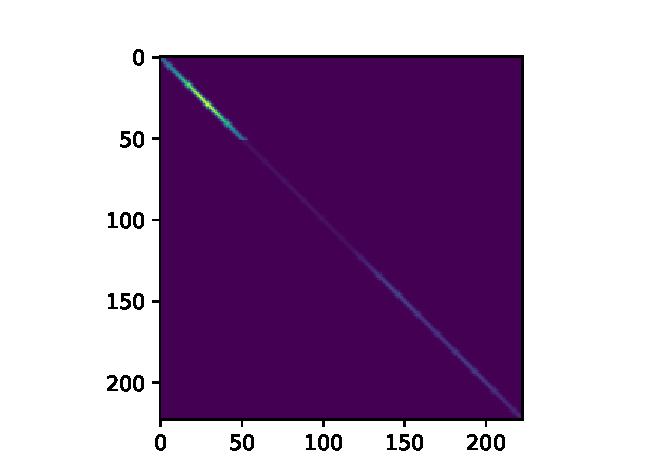
\includegraphics[width=\linewidth]{plots/Diagonal.pdf}
%     \caption{Example of the correlation matrix used in the likelihood function. The diagonal elements $\text{C}_{ij} = \delta_{ij}\sigma_{ij}^2$ correspond to the uncertainty of the data and the off-diagonal elements characterise the correlations between nearby detector pixels \citep[see][]{2015ApJ...812..128C}.}
%     \label{DiagonalMatrix}
% \end{figure}
\begin{figure}
	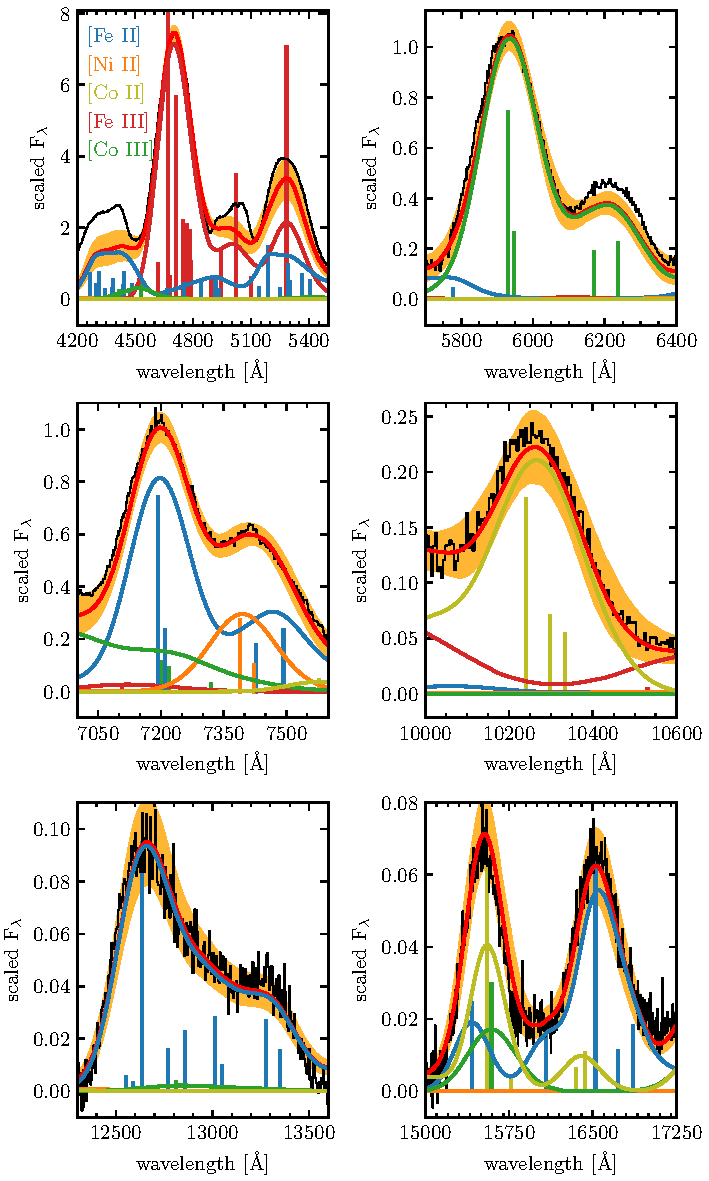
\includegraphics[width=\linewidth]{plots/example_fit.pdf}
    \caption{Example fit of SN\,2017bzc at +215\,days after B-band maximum. The individual panels highlight the ionic emission contributions to six features from the near-UV to the NIR. The strongest lines of each ion are indicated as vertical lines. The height of these lines shows their relative strengths. The flux of the spectrum was scaled to the 7155\,\AA\,peak. The observed spectrum is not corrected for extinction and redshift of the host. Instead, all model lines are extinguished and redshifted.}
    \label{ExampleFit}
\end{figure}

For each spectrum we can use the posterior distribution of the model parameters to compute line emissivities of all lines of singly and doubly ionized Fe, Ni and Co. In this work we use line ratios of [\ion{Ni}{II}] and [\ion{Fe}{II}]. \ion{Ni}{II} emission in the nebular phase can only be the result of the stable isotope $^{58}$Ni, as the radioactive material has long since decayed. Fe can be produced directly during the explosion as $^{54,56}$Fe or it can be the decay product of radioactive $^{55}$Co, $^{56}$Ni and $^{57}$Ni. The line ratio of [\ion{Ni}{II}] and [\ion{Fe}{II}] allows us to determine the mass fraction of neutron rich to radioactive material, which can be compared to predictions of explosion models. A similar study was performed for the NIR line ratio of the 1.547\,$\mu$m [\ion{Co}{II}] to the 1.533\,$\mu$m [\ion{Fe}{II}] line in \citet{2018A&A...620A.200F}. While the NIR nebular spectra are easier to model than the optical spectra, the mass ratio of \ion{Co}{II} to \ion{Fe}{II} changes with time and the number of spectra with NIR coverage is quite limited. In this work we want to make use of several decades of optical nebular phase spectroscopy to determine the distribution of the Ni/Fe abundance and compare our findings with predictions from explosion models.

\subsection{Calibration of optical spectra of SNe Ia}
\label{Calibration}
To determine the \ion{Ni}{II} / \ion{Fe}{II} mass ratio we compute the ratio of the $7378$\,\AA\, [\ion{Ni}{II}] and the 7155\,\AA\,[\ion{Fe}{II}] lines. The conversion of line emissivities to emitting masses requires further knowledge of the temperature and density of the emitting material. The one-zone-model employed in this study does not allow us to disentangle these two parameters even if we have both optical and NIR spectra. However, we find that the evolution of the ratio of the strongest \ion{Fe}{II} line in the NIR ($\lambda$12570) and optical ($\lambda$7155) is very similar across our sample of optical+NIR spectra. We fit a simple linear relation through our inferred data points (see Fig. \ref{FigureRatioNIR_VIS}). The uncertainties of the individual data points are uncorrelated, thus justifying the use of a simple Chi-Square likelihood
\small
\begin{equation}
    \ln p(y|t, \Delta y, m, b, \sigma) = -\frac{1}{2}\sum_n \left( \frac{(y_n -mx_n -b)^2}{s_n^2} + \ln(2\pi s_n^2)\right)
\end{equation}
\normalsize
where
\begin{equation}
    s_n^2 = \sigma_n^2 + \sigma^2(mx_n+b)^2.
\end{equation}
In this equation y and $\Delta y$ indicate the inferred values and uncertainties of the \ion{Fe}{II} 12570\AA\,to 7155\,\AA\,ratio for our sample, $m$ is the slope of the fit curve, $b$ is its intersect, and $\sigma$ is the intrinsic scatter of the population.
We add an intrinsic scatter term to the likelihood function that takes into consideration that our sample consists of many different objects. The uncertainty of the fit is then a combination of the uncertainty of slope and intersect and the intrinsic scatter term.
We find for the ratio of \ion{Fe}{II} 12570\AA\,to 7155\,\AA
\small
\begin{equation}
    \label{EquationNIROPT}
    \log\frac{F_{12570}}{F_{7155}} = -(1.65\pm0.07) + (0.0043\pm0.0002)\,d^{-1}\,\times t_{\text{exp}}[\text{days}]
\end{equation}
\normalsize
with an intrinsic scatter of 0.06\,dex around the best fit curve. The choice of the atomic data has only very weak consequences on the inferred NIR/VIS ratio. Translating the NIR/VIS ratio to temperatures/densities does rely on the atomic data, however. The atomic data used throughout this work is given in Table \ref{tab:AtomicData}.

Alone, the optical spectra of SNe Ia do not allow us to constrain the temperature and density of the emitting material in any meaningful way - we can obtain good fits for a wide range of temperatures and densities. However, we notice that for a given \ion{Fe}{II} 12570\AA\,to 7155\,\AA\,ratio only specific tracks in the temperature/density space are possible. The inference uncertainty of the NIR/VIS ratio translates into a curve with non-zero width in the temperature/density space. The measurement of the NIR/VIS line ratio is considered solid - no other strong lines are present in the 1.25\,$\mu m$ feature, and in the 7000\,\AA\,region only \ion{Co}{III} of the iron group elements has a somewhat weak contribution. By fitting many lines of singly and doubly ionized material at optical and NIR wavelengths we can also exclude the extremes in the temperature/density space (see grey shaded areas in Fig. \ref{FigureTemperatureDensity}). Each of the curves in Fig. \ref{FigureTemperatureDensity} corresponds to one value of the NIR/VIS ratio. We can thus determine the range of temperatures and densities of SNe Ia in the nebular phase with only optical spectra by enforcing that the \ion{Fe}{II} 12570\AA\,to 7155\,\AA\,ratio evolves as the red curve in Fig. \ref{FigureRatioNIR_VIS} with a 1-sigma uncertainty of 0.06\,dex. We add this constraint as a Gaussian prior into the likelihood function of our Bayesian fit model. 

\subsection{Determination of the Ni to Fe ratio}
Our model does not allow us to accurately compute emitting masses as the temperature dependence is too strong. A temperature difference of only a few hundred Kelvin can lead to an emitting mass that is different by a factor of a few. A more robust quantity is the mass ratio of ions of the same ionisation stage. Due to their similar emitting region \citep{2018MNRAS.477.3567M,2018A&A...620A.200F} the physical conditions of the ions (temperature and electron density) are similar. The mass ratio also negates the effect of the rather unknown distance to the SN host galaxy and significantly reduces the effect of the emitting temperature. 

% For the optical lines of [\ion{Fe}{II}] and [\ion{Ni}{II}] we cannot use the relation from \citet{1990MNRAS.245..570V}, which is an approximation for LTE conditions. The upper level energies of the ions in question are much higher for optical than NIR lines (\ion{Fe}{II}: E$_{upper}=8\,392$ cm$^{-1}$ for 15330\,\AA\,compared to E$_{upper}=15\,845$ cm$^{-1}$ for 7155\,\AA). Populations of levels responsible for optical transitions drop out of LTE early in the nebular phase, while the departure from LTE conditions is only a few percent for the low-lying levels responsible for NIR transitions even 400 days after the explosion.  \textcolor{blue}{Maybe add plot that shows the departure coefficients?}

For a given temperature and density we can directly infer the ratio of the number of emitting \ion{Fe}{II} and \ion{Ni}{II} ions required to match the observed flux ratio of the 7155\,\AA\, and 7378\,\AA\,lines. Temperatures and densities that yield a good fit can be found if a NIR spectrum is available. For spectra that lack this additional information we have to use the relation obtained in Section \ref{Calibration}. We discuss the additional uncertainties from using the fit relation instead of the full optical + NIR spectrum in Section \ref{NiFeTest}.


\begin{table}
	\centering
	\scriptsize
	\caption{Results of the ratio of the 12570\,\AA\,and 7155\,\AA\,lines of \ion{Fe}{II}, the M$_{\text{Co}}$\,/\,M$_{\text{Fe}}$ ratio and the M$_{\text{Ni}}$\,/\,M$_{\text{Fe}}$ ratio for the extended XShooter sample.}
	\label{tab:LineRatio}
    \begin{tabular}{lclccc}
    % F$_{12570\text{\AA}}$/F$_{7155\text{\AA}}$
    	\hline 
    	SN 		  & Ref$^a$ & Epoch & R$_{12570/7155}$ &	M$_{\text{Co}}$/M$_{\text{Fe}}$ & M$_{\text{Ni}}$/M$_{\text{Fe}}$\\
		\hline  
% 		SN\,2018aoz & TW & +126\,d & $0.145\pm0.021$ & 0.353$\pm$0.041\\
% 		SN\,2017fzw & TW & +177\,d & $0.141\pm0.011$ \\
		SN\,2015F   & TW & +181\,d & $0.173\pm0.16$ & 0.231$\pm$0.02 & 0.061$\pm$0.010\\
% 		SN\,2017fzw & TW & +202\,d & $0.141\pm0.011$\\
    	PSNJ1149  & M18 & +206\,d & $0.199\pm0.022$ & 0.152$\pm$0.012$^b$ & 0.044$\pm$0.011\\
    	SN\,2017bzc & TW & +215\,d & $0.211\pm0.044$ & 0.154$\pm$0.01 &0.035$\pm$0.009\\
        SN\,2015F   & TW & +225\,d & $0.241\pm0.018$ & 0.142$\pm$0.02 & 0.055$\pm$0.008\\
        SN\,2013ct  & M16 & +229\,d & $0.279\pm0.021$ & 0.103$\pm$0.010$^b$ & 0.037$\pm$0.006\\
        SN\,2015F   & TW & +239\,d & $0.325\pm0.022$ & 0.127$\pm$0.02 & 0.052$\pm$0.008\\
        SN\,2015F   & TW & +266\,d & $0.314\pm0.020$ & 0.097$\pm$0.01 & 0.055$\pm$0.009\\
        SN\,2013cs  & M16 & +303\,d & $0.486\pm0.029$ & 0.066$\pm$0.011$^b$ & 0.031$\pm$0.006\\
        SN\,2012cg  & M16 & +339\,d & $0.726\pm0.021$ & 0.051$\pm$0.005$^b$ & 0.038$\pm$0.006\\
        SN\,2012fr  & M16 & +357\,d & $0.947\pm0.048$ & 0.038$\pm$0.004$^b$ & 0.025$\pm$0.005\\
    	SN\,2013aa  & M16 & +360\,d & $1.00\pm0.068$ & 0.035$\pm$0.003$^b$ & 0.033$\pm$0.006\\
        SN\,2015F   & TW & +406\,d & $1.36\pm0.06$ & $-$ & 0.049$\pm$0.009\\
        SN\,2013aa  & M18 & +425\,d & $2.07\pm0.14$ & 0.025$\pm$0.003$^b$ & 0.035$\pm$0.007\\
        SN\,2012ht  & M16 & +433\,d & $1.87\pm0.11$ & 0.020$\pm$0.005 & 0.009$\pm$0.004\\
        % SN\,2017fzw & TW & +490\,d & $3.31\pm0.21$ & $-$ & 0.034$\pm$0.009\\
		\hline
	\end{tabular}
	\begin{flushleft}
         $^a$Source of the nebular spectrum: TW (This Work); M16 \citep{2016MNRAS.457.3254M}; M18 \citep{2018MNRAS.477.3567M}
         $^b$Result taken from \citet{2018A&A...620A.200F}
    \end{flushleft}
\end{table}
\begin{figure}
	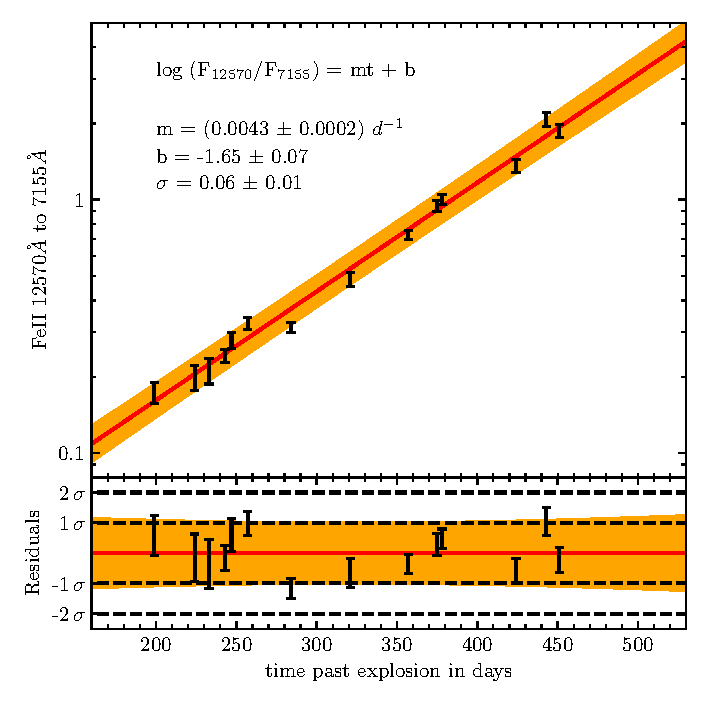
\includegraphics[width=\linewidth]{plots/FeII_NIR_VIS_Ratio.pdf}
    \caption{Inferred ratio of the \text{Fe\,\textsc{\lowercase{II}}} 12570\,\AA\,to 7155\,\AA\,lines as a function of time after explosion. The red line marks a linear fit to data of the form y = mt + b with intrinsic scatter $\sigma$. The orange shaded band indicates the $68\%$ confidence interval of the regression curve.}
    \label{FigureRatioNIR_VIS}
\end{figure}
\begin{figure}
	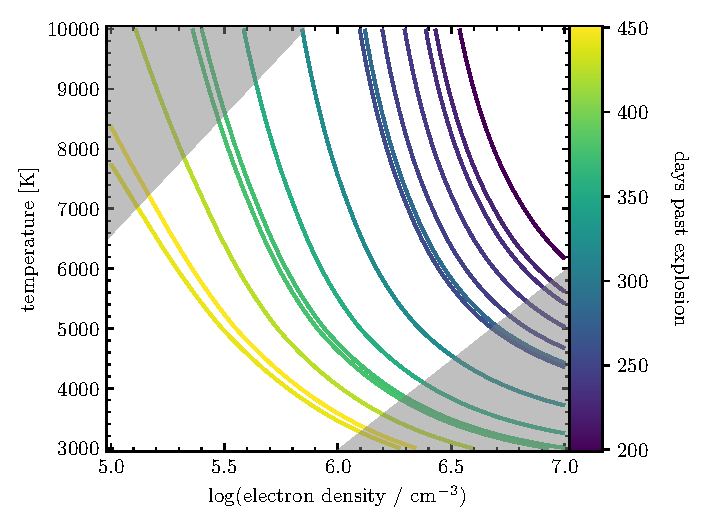
\includegraphics[width=\linewidth]{plots/TempDensDegeneracy.pdf}
    \caption{Allowed regions of the electron density and temperature for the SN Ia in our sample. Every curve corresponds to one value of the 12570\,\AA\,to 7155\,\AA\,\ion{Fe}{II} line ratio. The allowed region is evolving with time to lower temperatures and densities. The evolution of the density is in agreement with just homologous expansion of the ejecta. Colors indicate the epochs of the spectra. The grey shaded regions (high density + low temperature; low density + high temperature) are excluded by the fits to [\ion{Ni}{II}] and [\ion{Co}{II}].}
    \label{FigureTemperatureDensity}
\end{figure}
\begin{figure}
	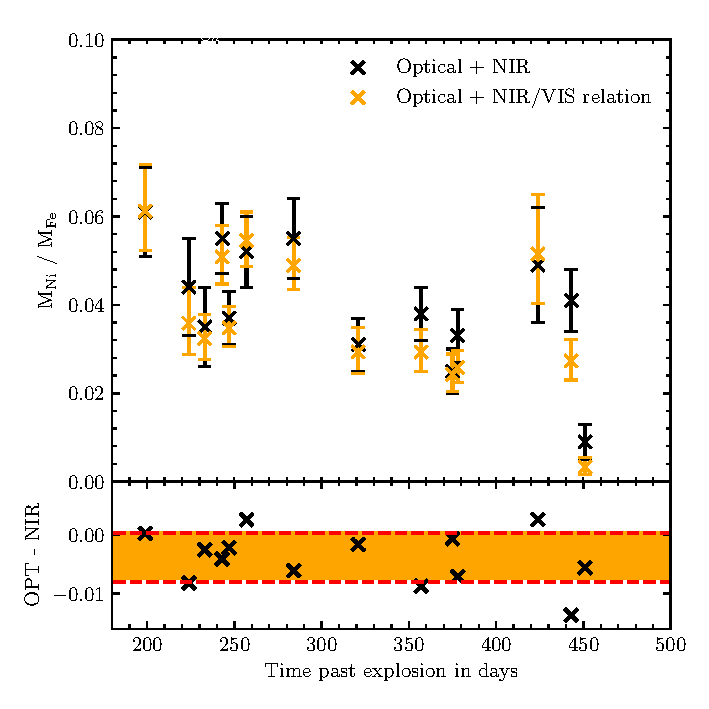
\includegraphics[width=\linewidth]{plots/NiFe_singly.pdf}
    \caption{Inferred mass ratio of \text{Ni\,\textsc{\lowercase{II}}} and \text{Fe\,\textsc{\lowercase{II}}} from optical and NIR spectroscopy. Black data points indicate that the \text{Fe\,\textsc{\lowercase{II}}} NIR/VIS ratio was directly inferred from a spectrum covering 4,000--20,000\,\AA. Orange data points indicate that only the optical part of the spectrum was used in conjunction with the relation from Fig.\,\ref{FigureRatioNIR_VIS} as a prior. We assume a rise time of $\sim 18$ days \citep{2011MNRAS.416.2607G} to compute the time after explosion. The bottom panel shows the systematic differences between the two methods -- optical spectra + the NIR/VIS relation (OPT) and fitting the full spectrum (NIR). The orange shaded band in the bottom panel marks the 68\% confidence interval of the systematic uncertainty $\sigma_{sys}=-0.0033^{+0.0037}_{-0.0041}$.}
    \label{NiOverFe}
\end{figure}
\begin{figure*}
	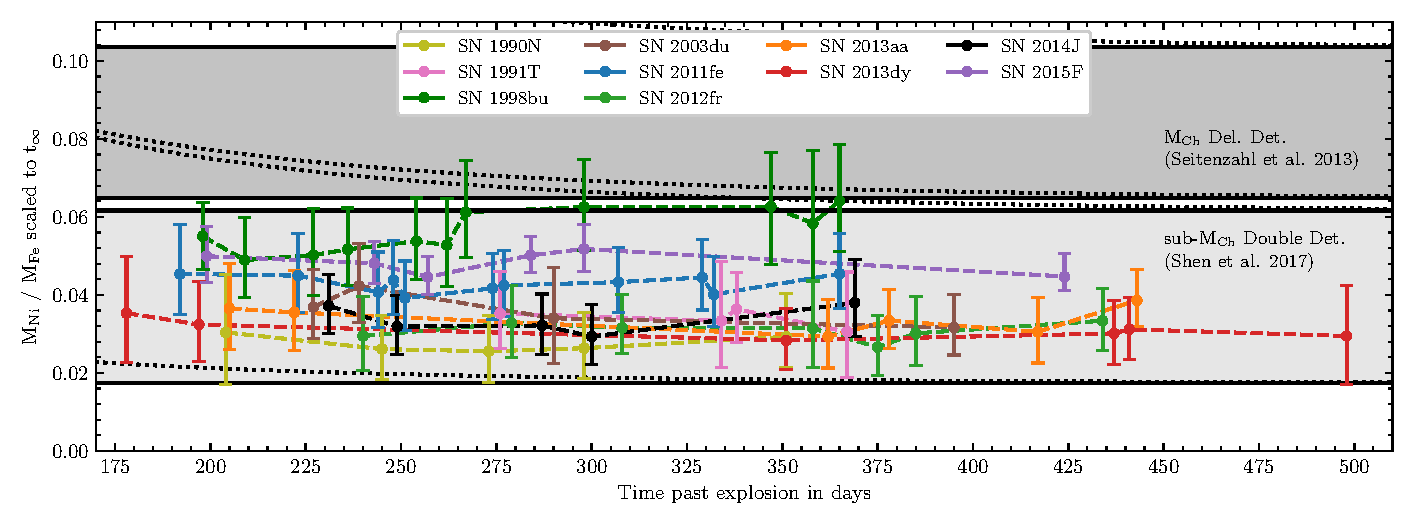
\includegraphics[width=\linewidth]{plots/NiFe_singly_multiplespectra.pdf}
    \caption{Inferred mass ratio of \text{Ni\,\textsc{\lowercase{II}}} and \text{Fe\,\textsc{\lowercase{II}}} for supernovae with multiple observations between 200 and 500 days after the explosion. Explosion model predictions and inferred data points were scaled to the Ni/Fe abundance at $t\rightarrow\infty$ to remove the time dependence of M$_{\text{Fe}}(t)$ in order to better illustrate the consistency of the method. We assume a rise time of $\sim 18$ days \citep{2011MNRAS.416.2607G} to compute the time after explosion. Same colors indicate multiple observations of the same supernova. Error bars represent the combined statistical fitting uncertainty and the systematic uncertainty from using the NIR/VIS relation if the spectrum only covers the optical wavelength region up to 1$\,\mu$m. Black dotted lines mark the model regions before the normalization to $t\rightarrow\infty$.}
    \label{NiOverFe_test_timesequences}
\end{figure*}
\begin{figure*}
	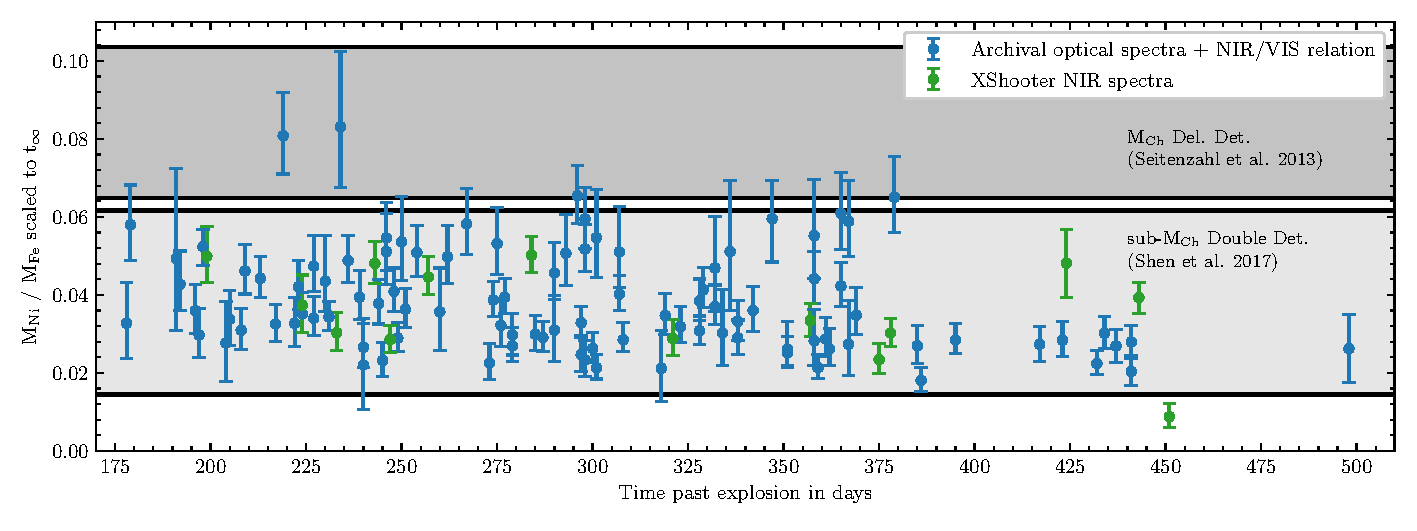
\includegraphics[width=\linewidth]{plots/NiFe_all_SNe.pdf}
    \caption{Inferred mass ratio of \text{Ni\,\textsc{\lowercase{II}}} and \text{Fe\,\textsc{\lowercase{II}}} from archival optical spectra and XShooter observations. Black datapoints indicate that the \text{Fe\,\textsc{\lowercase{II}}} NIR/VIS ratio was directly inferred from a spectrum covering 4,000--20,000\,\AA. Blue data points indicate optical nebular phase spectra that have been modelled using the relation from Fig.\,\ref{FigureRatioNIR_VIS} as a prior. Errorbars only indicate the statistical uncertainty from the fit. We assume a rise time of $\sim 18$ days \citep{2011MNRAS.416.2607G} to compute the time after explosion. The shaded bands display predictions of the Ni to Fe mass ratio from explosion model simulations. Inferred and predicted mass ratios were scaled to $t\rightarrow\infty$.}
    \label{NiOverFe_all}
\end{figure*}
\section{Discussion}
\subsection{The Fe$\,\textsc{II}$ NIR/VIS ratio}
In Section \ref{Calibration} we derived a relation between two of the strongest \ion{Fe}{II} lines that are observed in nebular spectra of SNe Ia. Our extended XShooter sample now contains 14 spectra of 9 different SNe. The ratio of the NIR 1.257\,$\mu$m and the 7155\,\AA\,lines evolves similarly for the objects in our sample. In physical terms, the ratio of these lines is a direct measure of the cooling and expanding Fe-rich ejecta. The relation does not depend on the collision strengths but only on the transition rates of \ion{Fe}{II}. These are well known, as can be seen from the match of the fit models and the observed spectra in regions where only \ion{Fe}{II} emission is present. Additionally, the \ion{Fe}{II} NIR/VIS relation as presented in this work is not just the result of a possible oversimplification of our one-zone model. It is obtained by effectively de-blending the lines of singly and doubly ionized iron, nickel and cobalt. It only depends on the total emission through the two lines. The assumed Gaussian line profile used in this work only has a marginal effect on the inferred values. More sophisticated explosion models should be able to reproduce the relation by integrating the flux of the 1.257\,$\mu$m and the 7155\,\AA\,lines over all emitting regions in the case of a multizone model.

\subsection{Robustness of the Ni/Fe ratio}
\label{NiFeTest}
In this section we test the robustness of the inferred Ni/Fe ratio. We test how the Ni/Fe ratio changes if we fit the optical part of the XShooter spectra with the relation from \ref{Calibration}. This allows us to estimate the systematic differences between the Ni to Fe ratio from XShooter and optical spectra. For well observed supernovae we can also test if the time evolution of the inferred ratio is consistent with the decay of radioactive iron-group elements (IGE).


\subsubsection{Fitting optical XShooter spectra with the NIR/VIS fit relation}
\label{TestNIRVIS_relation}
Using the inferred \text{Fe\,\textsc{\lowercase{II}}} 7155\,\AA\, to 12570\,\AA\,relation as a prior for spectra without the NIR we are adding a systematic uncertainty to the model. In this section we want to estimate the systematic uncertainty introduced by using the relation. For this reason we fit only the optical spectrum for each object in our XShooter sample and compare the obtained Ni/Fe ratio to the fit of the whole optical+NIR spectrum. The only change to the fitting procedure compared to the one for optical+NIR spectra is the omission of \ion{Co}{II}, which has no strong lines in the optical -- escpecially not close to the 7200\,\AA\,feature. It does therefore have no influence on the obtained value for the NIR/VIS ratio.

A large difference between the direct fit result of the optical+NIR spectrum and the optical spectrum + NIR/VIS prior would indicate that our method is not suitable for just optical spectra. We show the results of this comparison study in Fig. \ref{NiOverFe}. For most objects in the XShooter sample, the difference between the two methods is quite small. At later epochs we see stronger deviations, which are mostly due to the low number of spectra beyond 400 days, widening the NIR to VIS relation. The difference at these extremely late epochs on the large optical sample is negligible as only a very small fraction of optical spectra are affected. Most optical spectra were taken less than one year after the SN explosion. 

The use of the NIR/VIS relation as a prior does not imply that the posterior of the 12570\,\AA\,to 7155\,\AA\,line ratio for a given epoch t$_i$ has the same width as the fit curve in Fig. \ref{Calibration}. In general, fitting the optical spectrum with the use of the NIR/VIS relation does not necessarily prefer the same ratio as fitting the full optical and NIR spectrum. As a result, we obtain different posteriors for the density and temperature for the two fitting methods. It seems that the optical is more sensitive to different regimes of the electron density and temperature than the combined optical and NIR spectrum. On average, the use of the \text{Fe\,\textsc{\lowercase{II}}} 12570\,\AA\,to 7155\,\AA\, fit relation instead of the NIR spectrum leads to a systematic difference of $\sigma_{sys}=-0.0033^{+0.0037}_{-0.0041}$. The use of the NIR/VIS relation therefore results in mostly smaller M$_\text{Ni}$\,/\,M$_\text{Fe}$ ratios by about 0.0033 within the 68\% confidence interval. We consider this a systematic uncertainty that adds to the statistical uncertainty linearly.

The inferred electron densities and temperatures from fitting only the optical spectrum and using the NIR/VIS relation lead to a NIR spectrum that does not necessarily agree with the NIR data of our test sample. However, if we apply the method to our large optical sample we do not have the data to compare whether the NIR spectrum is in agreement. For this work we therefore treat the difference between the two methods as a systematic uncertainty that originates in the use of the NIR/VIS relation and which systematically yields lower values for the Ni to Fe ratio if applied to optical spectra. This systematic uncertainty is generally smaller than the statistical uncertainty from the fitting procedure.

\subsubsection{Time evolution of the Ni/Fe ratio}
Even though the amount of $^{58}$Ni produced in the explosion is fixed for a single object, the ratio of Ni/Fe can still change with time. This is due to Fe being the daughter product of $^{56}$Co decay, which at early times has not completely decayed yet. Only after $\sim300$\,days (4 $\times$ t$_{1/2}$) the Ni/Fe ratio remains almost constant. 

For supernovae that have several observations during the nebular phase we can test whether our method yields Ni to Fe ratios that can be explained by a single model. Effectively, this means that the slope of the data points should follow the theoretical explosion model predictions. In Fig. \ref{NiOverFe_test_timesequences} we normalize the Ni to Fe to the value at $t=t_\infty$ to make it easier for the reader to see the slope of the measured data points. A flat series of data points indicates that the evolution with time behaves just like radioactive decay of $^{56}$Ni:
% \newpage
\begin{equation}
    \frac{M_\text{Ni}}{M_\text{Fe}}= \frac{M_{^{58}\text{Ni}}}{M_{^{56}\text{Ni,t=0}}(1-e^{-\lambda t}) + M_{^{54,56}\text{Fe}}}
\end{equation}
The evolution of the Ni to Fe mass ratio for objects with multiple observations during the nebular phase is consistent with pure radioactive decay within the statistical uncertainties. A much shallower or steeper slope of the NIR/VIS ratio would lead to non-flat evolutionary curves of the Ni/Fe ratio. 
The only object that shows an evolution of the scaled Ni/Fe mass ratio is SN\,1998bu. Roughly 270 days past its B-band maximum the inferred Ni/Fe mass ratio increases by about 15\% and settles on this new value for the remaining observations. Such a behaviour could be the result of a light-echo contribution to the nebular spectrum, as was found for SN\,1998bu by \citet{2001ApJ...549L.215C}. 

% Our XShooter sample consists of 18 spectra of 11 different objects and includes both the low-end (SN\,2017fzw, SN\,2015F) and high-end (SN\,2012fr, SN\,2012cg) of the Phillips-relation. Of course, a sample with only 10 objects cannot be a perfect display of the distribution of normal SNe Ia. However, we do find a very similar evolution of the NIR/VIS ratio across our sample. If we assume that our sample is insufficient to fully characterise the NIR/VIS ratio relation, then this will affect our inferred Ni/Fe ratio. In this section we will systematically change the relation in both offset and slope, use the modified relation to fit the well observed SN\,2011fe and compare our inferred values for Ni/Fe.

\subsection{A possible contribution of Calcium at 7200\,\AA?}
\label{Catest}
The method presented in Section \ref{SectionModels} relies on the assumption that only [\ion{Fe}{II}] and [\ion{Ni}{II}] contribute to the 7200\,\AA\,feature. If emission from another ion (e.g. \ion{Ca}{II}])  contributes substantially to this feature, our measurement will be systematically wrong as the true contribution of Ni to the feature is lower than estimated from our model. Some NLTE radiative transfer calculations of SNe Ia in the nebular phase predict a non-negligible flux of \ion{Ca}{II}] emission at $\lambda\lambda$ 7291.5,  7323.9 \citep{2017ApJ...845..176B}. If the emitting region is a spherical shell at high velocities outside the iron core, the profile would be flat-topped. Such a plateau of \ion{Ca}{II}] emission would raise the overall flux level in the 7200\,\AA\,region without changing the characteristic double peaked shape of the feature.

We can test whether there is a contribution from other ions by fixing the strength of the \text{Ni\,\textsc{\lowercase{II}}} 7378\,\AA\,through the 1.939\,$\mu$m line. The relative strength of the two lines only depends on the extinction and the ratio of the transition rates, as they originate from the same upper level:
\begin{equation}
    \frac{F_{1.939\,\mu\text{m}}}{F_{7378\,\text{\AA}}} = \frac{A_{^2F_{7/2} - ^4F_{9/2}}(E_{^2F_{7/2}} - E_{^4F_{9/2}})}{A_{^2F_{7/2} - ^2D_{5/2}} (E_{^2F_{7/2}} - E_{^2D_{5/2}})} = 0.202
\end{equation}
The observed strength will depend on the extinction. Unfortunately, there is a strong telluric absorption band just bluewards of the 1.939\,$\mu$m line of [\ion{Ni}{II}]. The SNR in this region is only sufficiently high for a small number of objects in our XShooter sample.  \citet{2018A&A...619A.102D} investigated the [\ion{Ni}{II}] 1.939\,$\mu$m line for the nearby SN\,2014J.

The observations of SN\,2015F, one of the closest SNe in the last decade, can be used to further verify this method. We obtained 5 nebular phase XShooter spectra between +181 and +406 days after B-band maximum. The first four epochs (+181, +225, +239, +266 days after maximum) are of exceptional quality and clearly show the 1.939\,$\mu$m line. The observation at +406 days has a SNR that is insufficient to detect such a weak line, especially as it lies close to a telluric feature. SN\,2017bzc was farther away than SN\,2015F, but with an integration time of 10080\,s the [\ion{Ni}{II}] 1.939\,$\mu$m line can be seen in the +215\,d spectrum.

An overview of the model fits for each of these spectra is shown in Fig. \ref{SN2015F_NiII}. The 1.9\,$\mu$m feature has not been used to compute the fits. A significant contribution of \text{Ca\,\textsc{\lowercase{II}}} in the optical would lead to a much weaker 1.939\,$\mu$m line, which is in contradiction to our observations. A weak \text{Ca\,\textsc{\lowercase{II}}} contribution cannot be ruled out but its effect on the Ni/Fe mass ratio would be very limited. None of the objects with sufficiently high SNR in the 1.9\,$\mu$m region require any \ion{Ca}{II}]. While it is not impossible that some SNe Ia -- transitional objects such as the 86G-like or the faint 91bg-like -- exhibit Calcium emission in the 7200\,\AA\, region, the feature can be explained by only [\ion{Fe}{II}] and [\ion{Ni}{II}] for the normal and luminous population of SNe Ia.


\begin{figure*}
	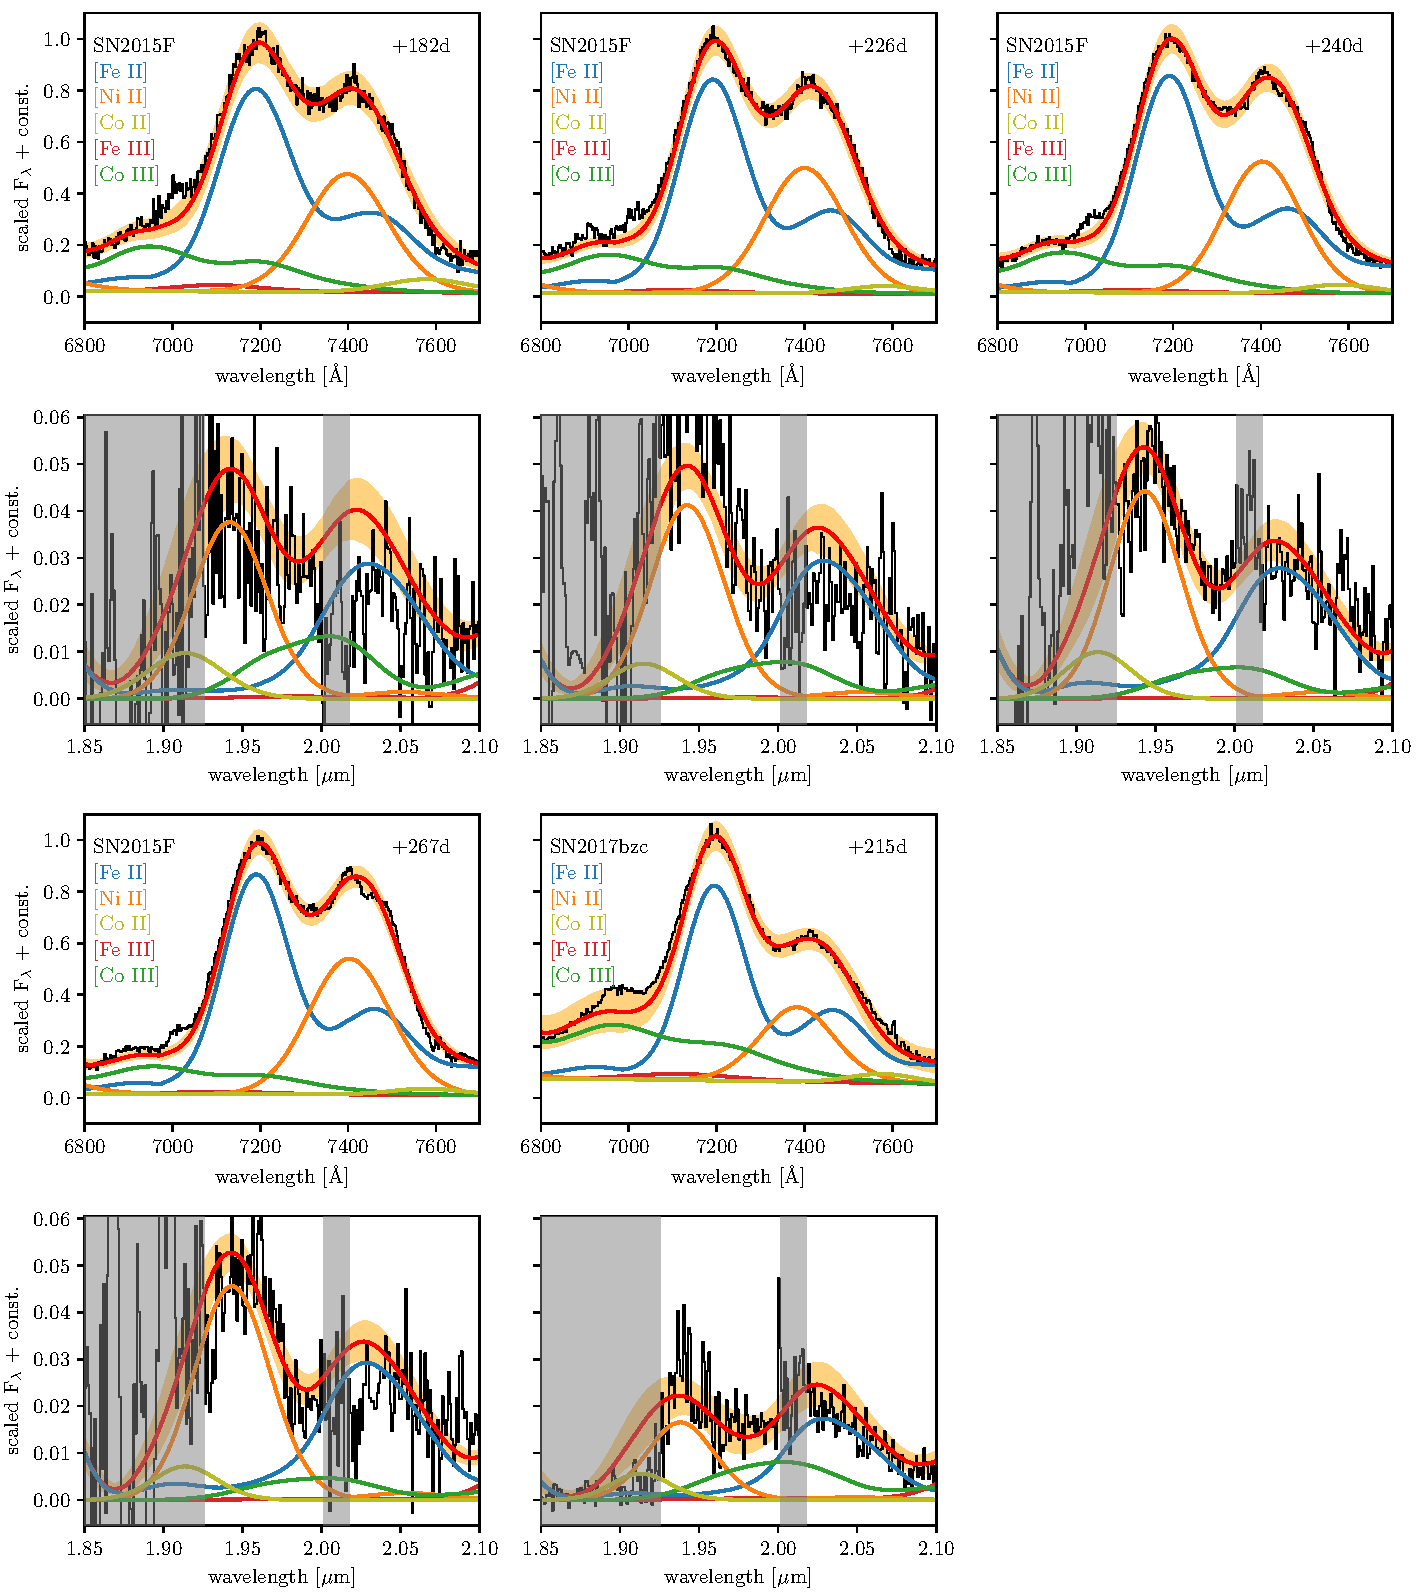
\includegraphics[width=\linewidth]{plots/NiII_OPT_NIR.pdf}
    \caption{Comparison between the \text{Fe\,\textsc{\lowercase{II}}} and \text{Ni\,\textsc{\lowercase{II}}} dominated regions in the optical at 7200\,\AA\,(top panel) and the NIR at $2\,\mu m$ (bottom panel) for four observations of SN\,2015F and one spectrum of SN\,2017bzc. The \text{Ni\,\textsc{\lowercase{II}}} lines at 7378\,\AA\, and 1.93\,$\mu$m originate in the same upper level a$^2$F$_{7/2}$ and have therefore a fixed line strength ratio that only depends on the ratio of their transition rates. For the atomic data adopted in this work the ratio of the 1.93\,$\mu$m to the 7378\,\AA\, line is 0.202. In the plots the ratio of the two lines is different because of two effects: The optical \ion{Ni}{II} feature is a blend of several lines and the flux density is lower at longer wavelengths. Regions of extremely low atmospheric transmission are shaded in grey.}
    \label{SN2015F_NiII}
\end{figure*}

\subsection{M$_\text{Co/Fe}$ from the extended XShooter sample}
% \textcolor{blue}{SN\,2015F has high Ni/Fe ratio, normal Co/Fe ratio at early times. Maybe it didn't produce any stable iron? This would increase the Ni/Fe ratio. The 57Ni wouldn't show up at early times even if significant amounts were produced, thus falling right on the 56Ni decay curve in the Co/Fe ratio. Maybe stable iron wasn't heated in this SN? But it should've been produced in the neutron rich zone of the explosion... Maybe ask Ivo Seitenzahl about this?}

The additional observations can be used to further the work described in \citet{2018A&A...620A.200F}. As has been noted by several authors \citep{2018MNRAS.477.3567M, 2018A&A...620A.200F}, the singly ionized lines of Fe, Ni and Co exhibit the same line shift and width. The same holds true for the two additional SNe with nebular phase XShooter observations presented in this work. It is therefore reasonable to assume that the singly ionized species are co-located in the ejecta and share the physical excitation conditions -- temperature and density. Our updated model allows us to directly compute the Co to Fe mass ratio without having to use LTE approximations. The effect, however, is quite limited for the NIR lines in question ($<\,5\%$). 

Fig. \ref{CoOverFe} displays a comparison of the new observations with the ones from \citet{2018MNRAS.477.3567M}. We find that the three new objects (SN\,2012ht, which was not included in the sample of \citeauthor{2018A&A...620A.200F} \citeyear{2018A&A...620A.200F}, SN\,2015F, SN\,2017bzc) have a M$_{\text{Co}}$\,/\,M$_{\text{Fe}}$ ratio that is consistent with sub-M$_{\text{Ch}}$ explosions. Only the spectrum of SN\,2012ht allows us to probe the $^{57}$Ni content in the ejecta as all other spectra are significantly younger than 300 days. For them, the ratio instead is a measure of the fraction of stable iron ($^{54,56}$Fe) to radioactive iron ($^{56}$Ni decay products). 
\begin{figure*}
	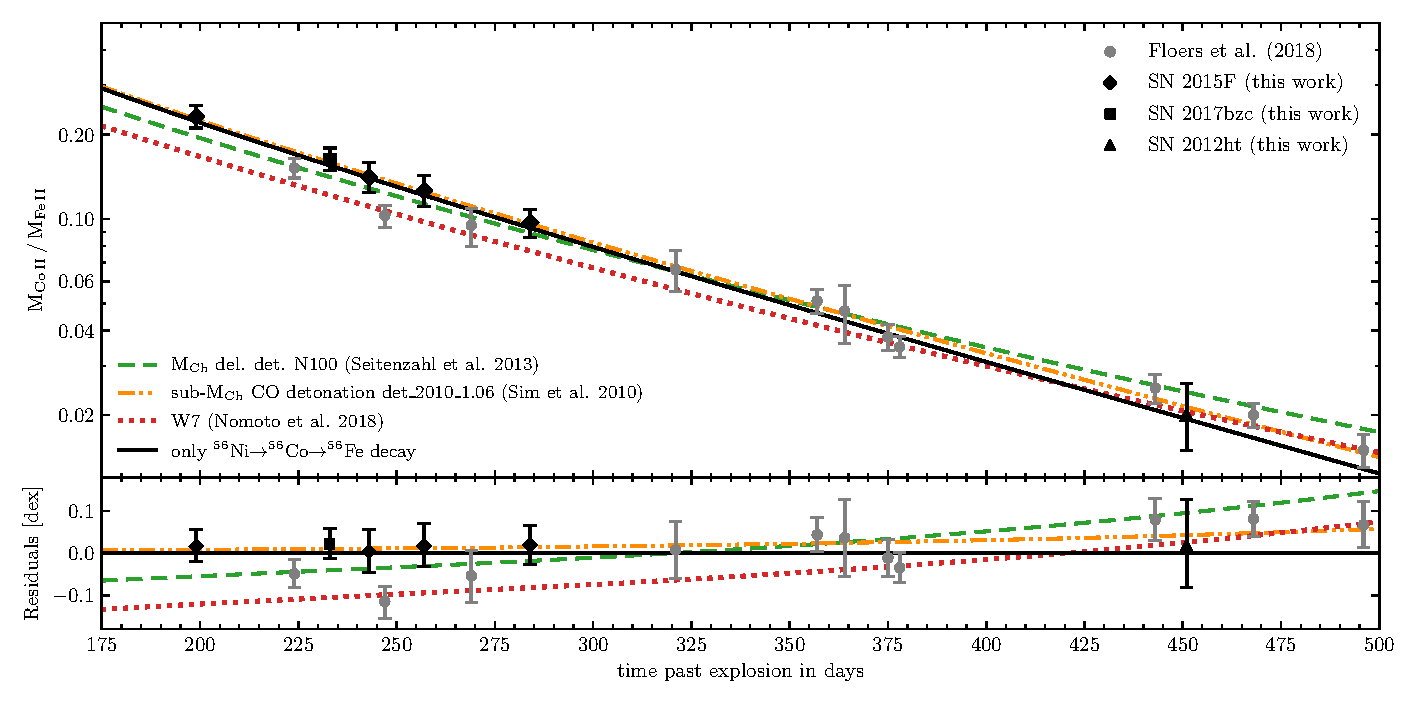
\includegraphics[width=\linewidth]{plots/MFeCo.pdf}
    \caption{Evolution of the inferred $\mathrm{M_{\ion{Co}{II}}\,/\,M_{\ion{Fe}{II}}}$ ratio with time for the extended XShooter sample. We assumed a rise time of 18 days \citep{2011MNRAS.416.2607G}. The error bars reflect the $68\%$ posterior interval of the mass ratio. The colored lines show the expected mass ratio $\mathrm{M_{Co}\,/\,M_{Fe}}$ of the M$_{\text{Ch}}$ delayed-detonation model `N100' \citep[][green]{2013MNRAS.429.1156S}, the sub-M$_{\text{Ch}}$ CO detonation model `det\_2010\_1.06' \citep[][orange]{2010ApJ...714L..52S} and the M$_{\text{Ch}}$ `W7 Z$_\odot$' model \citep[][red]{2018SSRv..214...67N}. The black line is not a fit to the data and represents the $\mathrm{M_{Co}\,/\,M_{Fe}}$ ratio assuming only radioactive decay from $^{56}$Ni to $^{56}$Co to $^{56}$Fe. Grey data points are from \citet{2018A&A...620A.200F}. Black data points are from the newly published objects in this work (SN\,2015F and SN\,2017bzc). The bottom panel shows the residuals normalized to the pure $^{56}$Ni to $^{56}$Co to $^{56}$Fe decay.}
    \label{CoOverFe}
\end{figure*}
\subsection{M$_\text{Ni/Fe}$ from archival optical spectra}
The evolution of the NIR/VIS lines of \ion{Fe}{II} allows us to model nebular spectra that cover only the optical wavelength range. We collected X spectra of Y SNe Ia at epochs $>\,170$ days after B-band maximum that have adequate SNR. A full list of all observations used for this study is given in Table \ref{TableSpectraOverview}. 
The spectra are modelled as described in Section \ref{SectionModels}. For SNe which have multiple observations in the nebular phase we combine the inferred mass ratios. We report the inferred scaled Ni/Fe mass ratio in \ref{TableSpectraOverview}. No corrections (e.g. fitting optical + NIR spectra vs only optical spectra; Section \ref{TestNIRVIS_relation}) have been applied to the inferred values. An overview of all objects (XShooter + archival) in our sample is given in Fig. \ref{NiOverFe_all}. We find that the majority of SNe exhibit Ni/Fe mass ratios below 0.05.

A similar study was conducted by \citet{2018MNRAS.477.3567M} for 8 objects in their XShooter sample. The same objects are also included in this work, however, a different method for the determination of the abundance ratio is used. Instead of modelling the full spectrum, \citet{2018MNRAS.477.3567M} restrict themselves to the $7200\,$\AA\,[\ion{Fe}{II}] and [\ion{Ni}{II}] dominated region. To convert the ratio of the LTE line fluxes to an abundance ratio of nickel and iron, they use average departure coefficients of a W7 model \citep{1984ApJ...286..644N,2018SSRv..214...67N} at 330\,days from \citet{2015ApJ...814L...2F}. As this model does not allow a determination of the temperature of the emitting material, \citet{2018MNRAS.477.3567M} assume temperatures similar to those of \citet{2015ApJ...814L...2F} between 3,000 and 8,000\,K.

The inferred abundance ratio of Ni and Fe from \citet{2018MNRAS.477.3567M} and this work deviate by about 1.5 $\sigma$ for the same objects. The differences are mainly due to the placement of the (pseudo-)continuum across the 7200\,\AA\,region, leading to a different line ratio of \ion{Fe}{II} 7155\,\AA\,and \ion{Ni}{II} 7378\,\AA. In this work we opted for a conservative continuum placement as most of it can be explained by a blend of weak lines of other singly and doubly ionized iron group ions (e.g. [\ion{Co}{III}], [\ion{Fe}{III}]). The departure coefficients corresponding to the allowed range of temperatures and densities (see Fig. \ref{FigureTemperatureDensity}) of the emitting material are in good agreement with the ones used by \citet{2018MNRAS.477.3567M}. The use of the \ion{Fe}{II} NIR/VIS relation allows us to better constrain the allowed range of the physical parameters of the singly ionized ejecta, leading to reduced uncertainties compared to \citet{2018MNRAS.477.3567M}. We want to emphasise that both works make use of the same atomic data for the ions in question.
\begin{figure}
	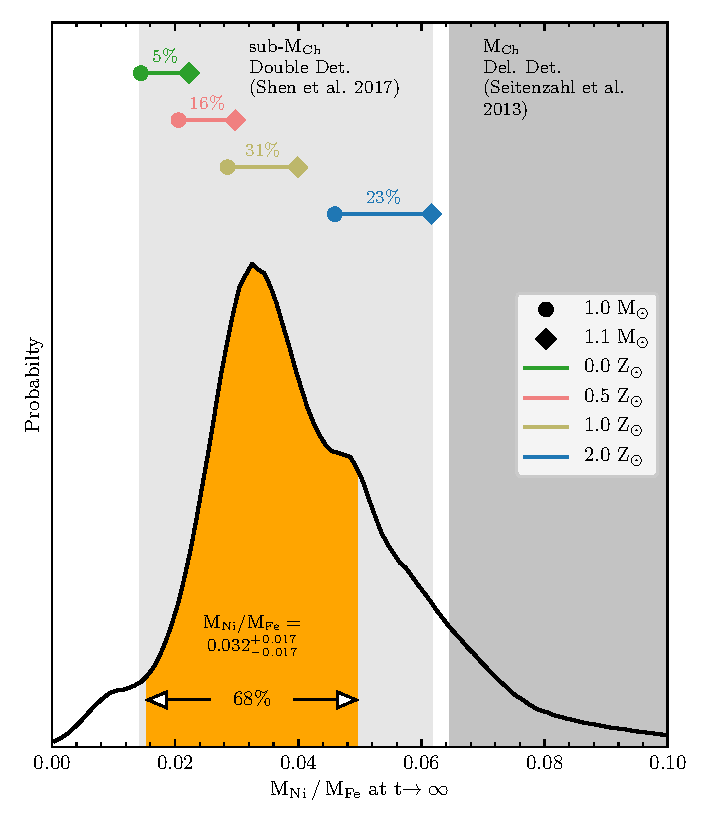
\includegraphics[width=\linewidth]{plots/NiFe_Distribution.pdf}
    \caption{The distribution of the Ni/Fe ratio at $t\rightarrow\infty$ from all available nebular phase spectra (see Table \ref{TableSpectraOverview}). The Ni/Fe ratio from only optical spectra was corrected according to Section \ref{TestNIRVIS_relation} by $\sigma_{sys}=-0.0033^{+0.0037}_{-0.0041}$. The results for SNe with multiple observations were combined so that every supernova in the sample contributes equally to the shown distribution - irrespective of the number of spectra. For each unique SN we drew 100\,000 samples from the posterior distribution of the Ni/Fe mass ratio. The orange shaded region indicates the region containing 68\% of the posterior probability density. Grey bands indicate predictions from sub-M${\text{Ch}}$ (left) and M${\text{Ch}}$ (right) explosion models. For sub-M${\text{Ch}}$ explosions we also show the range of models for 4 progenitor metallicities and their enclosed fraction of the posterior distribution of our sample.} 
    \label{NiFe_Distribution}
\end{figure}
\subsection{Implications on the explosion mechanism}

\label{Implications}The various theoretical explosion models of SNe Ia predict different amounts of neutron rich material. In M$_{\text{Ch}}$ explosions the amount of synthesized neutron-rich material is determined by two processes: \textit{Carbon simmering} and \textit{neutron-rich burning}:
 
\textit{Carbon simmering} occurs when a white dwarf accretes slowly towards the M$_{\text{Ch}}$. Temperatures in the center become high enough to ignite carbon, but no thermonuclear runaway happens due to a large convective core that allows for cooling through escaping neutrinos \citep{2004ApJ...607..921W, 2004ApJ...616.1102W, 2008ApJ...678.1158P}. The burning of carbon leads to mostly $^{13}$N and $^{23}$Na, which can subsequently capture electrons which further increases the neutron excess \citep{2008ApJ...677..160C, 2016ApJ...825...57M}.

\textit{Neutron-rich burning} to NSE can shift the equilibrium away from $^{56}$Ni to more neutron-rich isotopes ($^{54,56}$Fe, $^{57,58}$Ni, $^{55}$Mn) \citep{1999ApJS..125..439I, 2000ApJ...536..934B}. Just before the explosion, the high central density of the progenitor white dwarf leads to neutronisation through electron capture in the densest region. Neutron-rich NSE burning is only possible if there is a neutron excess in the NSE burning central region. 

In sub-M$_{\text{Ch}}$ models such processes are not possible as their progenitors cannot reach the required central densities and temperatures. However, an overabundance of neutrons in a high metallicity progenitor can still lead to the production of neutron-rich IGE \citep{2003ApJ...590L..83T}. The fraction of neutron rich to normal material can cover a wide range of values - from close to zero for $Z=Z_\odot$ to that of M$_{\text{Ch}}$ explosions at several times solar metallicity \citep{2018ApJ...854...52S}. It remains to be seen whether such extremely-high metallicity progenitors really exist. 

In this work we are interested in the composition of the iron-rich ejecta of SNe Ia. Theoretical explosion models contain the following isotopes in the central region:
\begin{itemize}
    \item[a)] $^{56}$Ni, which is the most abundant radioactive isotope and responsible for the heating of the ejecta. It decays within a few days ($t_{1/2}=6.075\,$d) to $^{56}$Co, which in turn decays ($t_{1/2}=77.2\,$d) to stable $^{56}$Fe. $^{56}$Ni can be produced in NSE (Nuclear Statistical Equilibrium) without an overabundance of neutrons (Y$_e=0.5$) or high densities. In our analysis, we treat $^{56}$Ni as a reference point and give other abundances in fractions of the $^{56}$Ni mass.   
    \item[b)] $^{57}$Ni, which decays with $t_{1/2}=1.48\,$d to $^{57}$Co. The decay of $^{57}$Co to stable $^{57}$Fe is slower ($t_{1/2}=271.74\,$d) than the decay of $^{56}$Co, so it can power the light curve at later epochs. Roughly 1000\,days after the explosion energy deposition from $^{57}$Ni decay overtakes the energy deposition from $^{56}$Ni. Most sub-M$_{\text{Ch}}$ explosions models predict an abundance M$_{^{57}\text{Ni}}$/M$_{^{56}\text{Ni}}$\,<\,2\,\%, while M$_{\text{Ch}}$ explosions predict >\,2\,\%.
    \item[c)] stable $^{54,56}$Fe that is directly synthesized in the explosion and not a daughter product of radioactive decay. M$_{\text{Ch}}$ explosions produce M$_{^{54,56}\text{Fe}}$/M$_{^{56}\text{Ni}}$\,>\,10\,\%, while most sub-M$_{\text{Ch}}$ models have M$_{^{54,56}\text{Fe}}$/M$_{^{56}\text{Ni}}$\,<\,10\,\%.
    \item[d)] stable $^{58}$Ni which is synthesized in the explosion. Sub-M$_{\text{Ch}}$ explosions contain M$_{^{58}\text{Ni}}$/M$_{^{56}\text{Ni}}$\,<\,5\,\% and M$_{\text{Ch}}$ explosions have M$_{^{58}\text{Ni}}$/M$_{^{56}\text{Ni}}$ between 8 and 12\,\%. 
\end{itemize}
We focus on the neutron-rich, stable $^{58}$Ni. The presence of a signature line close to $7378$\,\AA\,reveals that at least some amount of $^{58}$Ni can be found in all normal SNe Ia observed so far. As shown in Fig. \ref{SN2015F_NiII} the 7200\,\AA\,feature can be explained by a blend of mainly [\ion{Fe}{II}] and [\ion{Ni}{II}]. In principle there will also be varying amounts of stable iron produced during the explosion, but this contribution to the total iron mass is hard to disentangle from the overwhelming fraction of daughter products of radioactive $^{56}$Co. 

The observed spectra are fit well with our emission model. By using the relation from Section \ref{Calibration} we can compute the Ni/Fe ratio. At early times the ratio is still evolving with time as not all the $^{56}$Co has decayed to $^{56}$Fe yet. At late times (>250 days) the ratio remains constant. We find a large spread of Ni/Fe ratios, ranging from 0.02 to 0.08 within the 95\% confidence interval. We do not find any objects for which we can exclude the contribution of Ni to the nebular phase spectrum. 

Our results are in good agreement with sub-M$_{\text{Ch}}$ explosions of solar- to super-solar metallicity progenitors. Only one object (SN\,2012ht) has a Ni to Fe ratio that is consistent with explosion predictions from zero-metallicity sub-M$_{\text{Ch}}$ white dwarfs. There are only few calculations of non-zero metallicity sub-M$_{\text{Ch}}$ explosions \citep{2010ApJ...714L..52S, 2018ApJ...854...52S}. Our data are consistent with both sub-M$_{\text{Ch}}$ detonations and double detonations, but they do not allow us to distinguish between these two scenarios. 

We find a few objects which have Ni/Fe abundances consistent with nucleosynthetic predictions of exploding M$_{\text{Ch}}$ white dwarfs. However, we do not find separate populations but instead the distribution displays a tail of objects which have high Ni/Fe abundances. The abundance distribution of objects which have nebular phase observations peaks at M$_{\text{Ni}}$\,/\,M$_{\text{Fe}}$ = 0.032 with an $68\%$ confidence region between 0.015 and 0.049. $85\,\%$ of the total probability density falls within the shaded band of sub-M$_{\text{Ch}}$ explosion predictions. Only $9\,\%$ of the total probability lies in the range of M$_{\text{Ch}}$ delayed-detonation predictions. 

For sub-M$_{\text{Ch}}$ we can compare our resulting distribution to explosion yields of progenitors with different masses and metallicities. Progenitors with masses of 0.9\,M$_\odot$ or less do not produce enough $^{56}$Ni ($<\,0.3\,$M$_\odot$) to explain the brightness of normal SN Ia and are thus discarded for this comparison. The overlap between the range of yields from $1.0\,$M$_\odot$ to $1.1\,$M$_\odot$ progenitors with our inferred Ni/Fe distribution is shown in Fig. \ref{NiFe_Distribution}. We find good agreement with progenitors between 0.5 and 2 Z$_\odot$. 

%If we assume that the population of normal SNe Ia is the result of double detonations \citep{2018ApJ...854...52S} we can estimate the metallicity of the progenitor population. We find \textcolor{blue}{a progenitor metallicity of Y$_{e}$=?}.
% \begin{figure*}
% 	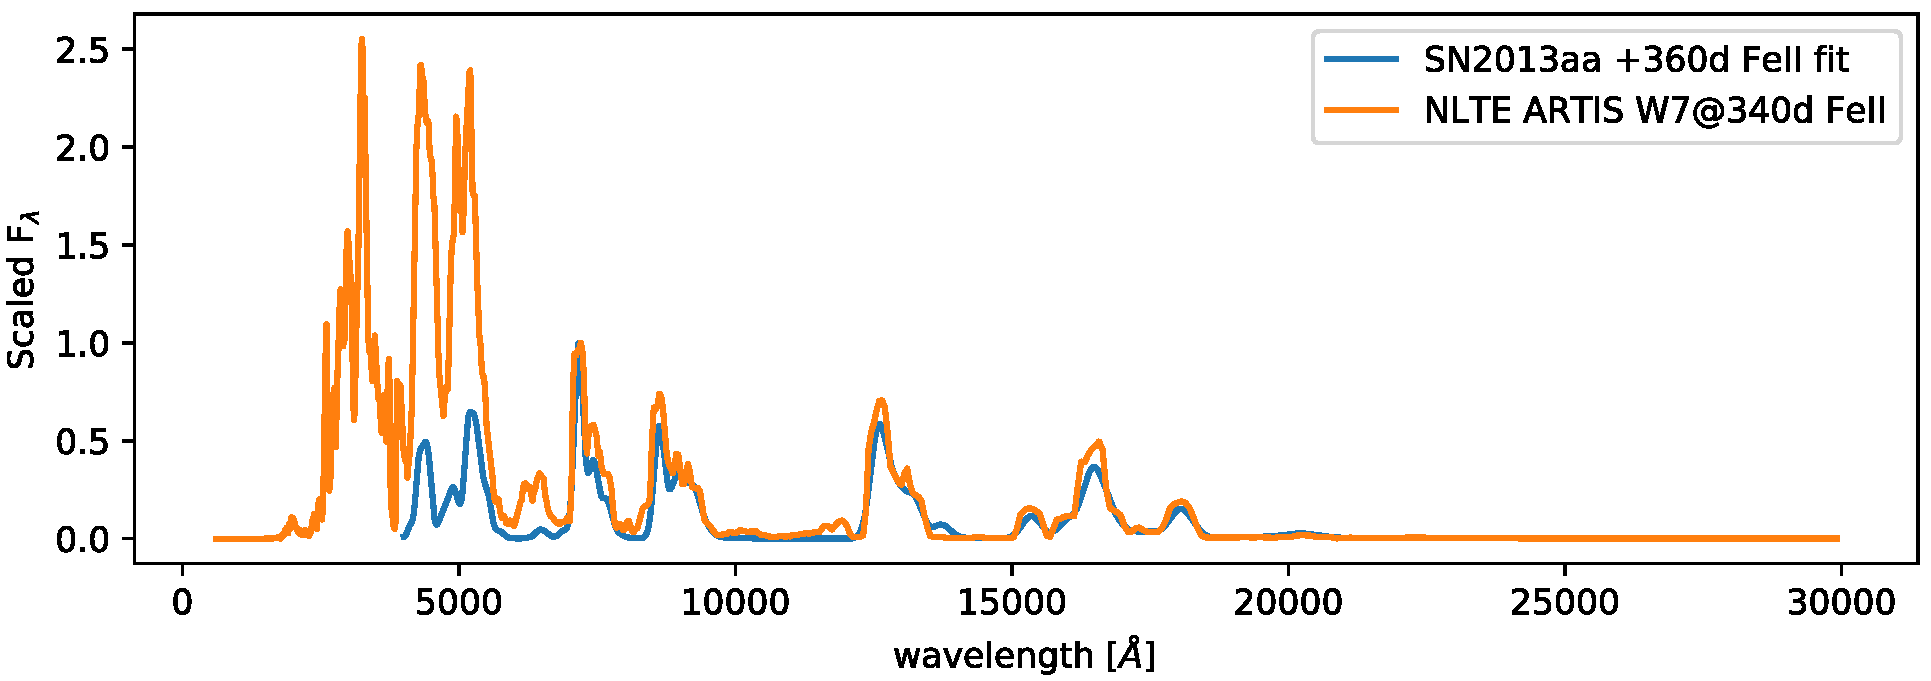
\includegraphics[width=\linewidth]{plots/Comparison_ARTIS_OneZone.pdf}
%     \caption{}
%     \label{FigureArtis_OneZone}
% \end{figure*}
% \subsection{Validity of the one-zone model}

\section{Conclusions}
In this work we have presented an extensive analysis of the 7200\,\AA\,feature in nebular spectra of SNe Ia. The feature which is composed of thermal emission of \ion{Fe}{II} and \ion{Ni}{II} can be seen in every single SN Ia observed so far, however, the relative contributions of the two ions to the feature can vary between different objects. We presented an extension to the method from \citet{2018A&A...620A.200F} that allows us to model the full optical and NIR spectrum and which takes into account the model imperfections. We applied the model to an extended sample of XShooter nebular phase spectra, of which 5 were previously unpublished. We found that the ratio of two strong \ion{Fe}{II} lines -- one in the NIR (12570\,\AA) and one in the optical (7155\,\AA) -- evolves with time in a straightforward manner. We have shown that we can use the evolution of these lines to constrain the previously unknown temperature and density in optical spectra. We applied the fitting method not only to the XShooter sample, but also to more than 100 optical archival spectra. This allows us to determine the distribution of the Ni/Fe ratio for all spectra in our sample, and compare the results to explosion model predictions. 
Our main results are:
\begin{itemize}
    \item[i)] The \ion{Fe}{II} emission in the nebular phase can be described by purely thermal forbidden line emission, and it is in agreement with an expanding and cooling nebula. 
    \item[ii)] The strongest [\ion{Fe}{II}] lines in the NIR and at optical wavelengths evolve with time, and the evolution seems to be very homogeneous across our sample. We obtained a relation that describes the evolution of this line ratio. The ratio does not depend on the atomic data. The evolution of the \ion{Fe}{II} lines can be used to test more sophisticated spectral synthesis calculations of explosion model predictions -- spectra that have been computed from explosion models need to be able to reproduce this relation.
    \item[iii)] The 7200\,\AA\,feature only contains \ion{Fe}{II} and \ion{Ni}{II} in normal SNe Ia. A contribution of \ion{Ca}{II} to this feature would have to be very limited in strength. We used the 1.939\,$\mu$m line to constrain the 7378\,\AA\,line for SN\,2015F and SN\,2017bzc as these two lines originate from the same upper level. We find no evidence that \ion{Ca}{II} emission is required to reproduce the 7200\,\AA\,feature.
    \item[iv)] For all objects in the extended sample of more than 100 nebular phase spectra we find that the lines of singly ionized \ion{Fe}{II} and \ion{Ni}{II} have similar widths and shifts and thus come from the same emitting region and share the same physical conditions. For objects for which NIR spectra are available we can extend this claim to \ion{Co}{II} as well. 
    \item[v)] The display of more than 100 nebular phase spectra shows a large variety in the relative strengths of the \ion{Fe}{II} and \ion{Ni}{II} lines in the 7200\,\AA\,feature. Translating the relative line strengths into a mass ratio of the singly ionized species results in a distribution which is expected from mainly sub-M$_{\text{Ch}}$ explosions.% with metallicities of the progenitor white dwarf between \textcolor{blue}{insert Y$_{e}$ here}.
    \item[vi)] We do not find separate populations of sub-M$_{\text{Ch}}$ and M$_{\text{Ch}}$ explosions. However, the high abundance tail of the distribution extends into the M$_{\text{Ch}}$ regime. 9\% of the total probability distribution lies within the M$_{\text{Ch}}$ predictions of the Ni/Fe abundance.
    %\item[vii)] Even if we massively underestimated the systematic uncertainties of the Ni/Fe mass ratio (e.g. uncertain atomic data) we find no evidence that there are several populations of progenitor systems/explosion scenarios. 
    %\item[viii)] Zero-metallicity sub-M$_{\text{Ch}}$ models can be excluded as the main explosion channel as we see emission from stable Ni during the nebular phase in all normal SNe Ia with quantities of stable Ni that are in conflict with such models.
\end{itemize}
\section*{Acknowledgements}
We thank the staff at the Paranal observatory. This research would not be possible without their efforts in supporting service mode observing. This research has made use of the NASA/IPAC Extragalactic Database (NED) which is operated by the Jet Propulsion Laboratory, California Institute of Technology, under contract with the National Aeronautics and Space Administration. This work made use of the Heidelberg Supernova Model Archive (HESMA), https://hesma.h-its.org. AF acknowledges the support of an ESO Studentship. 

This research made use of Astropy, a community-developed core Python package for Astronomy \citep{2013A&A...558A..33A, 2018AJ....156..123A}, as well as numpy \citep{Walt:2011:NAS:1957373.1957466}, scipy \citep{scipy}, pandas \citep{mckinney-proc-scipy-2010} and matplotlib \citep{doi:10.1109/MCSE.2007.55}.
%%%%%%%%%%%%%%%%%%%%%%%%%%%%%%%%%%%%%%%%%%%%%%%%%%

%%%%%%%%%%%%%%%%%%%% REFERENCES %%%%%%%%%%%%%%%%%%

% The best way to enter references is to use BibTeX:

\bibliographystyle{mnras}
\bibliography{bibliography} % if your bibtex file is called example.bib


% Alternatively you could enter them by hand, like this:
% This method is tedious and prone to error if you have lots of references
% \begin{thebibliography}{99}
% \bibitem[\protect\citeauthoryear{Author}{2012}]{Author2012}
% Author A.~N., 2013, Journal of Improbable Astronomy, 1, 1
% \bibitem[\protect\citeauthoryear{Others}{2013}]{Others2013}
% Others S., 2012, Journal of Interesting Stuff, 17, 198
% \end{thebibliography}

%%%%%%%%%%%%%%%%%%%%%%%%%%%%%%%%%%%%%%%%%%%%%%%%%%

%%%%%%%%%%%%%%%%% APPENDICES %%%%%%%%%%%%%%%%%%%%%

\appendix

\section{Overview of nebular spectra }
\begin{table*} 
    \caption{Overview of spectra in our sample.}
    \label{TableSpectraOverview}	
    \centering 
    \scalebox{0.95}{
	\begin{tabular}{l c c cccccccc} 
    \hline
    \hline 
    \centering 
    Supernova & Subtype & E$(B-V)$ & z & Date of max.& Epoch & Telescope & Instrument &  Ref & Ref & M$_{\text{Ni}}$\,/\,M$_{\text{Fe}}$\\
              &         & (mag)    &   &             &       &           &            & Spec & Ext &  ($t\rightarrow\infty$) \\
    \hline  
    SN\,1986G  & 86G-like  & $0.89$  & 0.001825 & 11 May 1986  & +257   & ESO-3.6m & EFOSC2-3.6      & 1 & 34 & $^{+}_{-}$ \\ 
             &           &         & 0.001825 & 11 May 1986  & +324   & ESO-3.6m & EFOSC2-3.6      & 1 & & $^{+}_{-}$ \\ 
    % SN\,1989B  & Ia-norm   & $0.40\pm0.03$ & 0.002425 & 06 Feb 1989  & +154   & Lick-3m & UV-Schmidt       & 2 & 2  \\ 
    % SN\,1989M  & Ia-norm   & $0.0351\pm0.0007$     & 0.005060 & 07 July 1989 & +147   & Lick-3m & UV-Schmidt       & 3 & -  \\
    % SN\,1990N  & Ia-norm   & $0.0223\pm0.0002$ & 0.003395 & 10 July 1990 & +160.6 & Lick-3m & UV-Schmidt       & 3 & -  \\
    SN\,1990N  & Ia-norm   & $0.0223$ & 0.003395 & 10 July 1990 & +186   & WHT-4.2m & FOS-2           & 4 &-& 0.027$^{+0.011}_{-0.010}$\\
             &           &          &          &              & +227   & WHT-4.2m & FOS-2           & 4 & & 0.023$^{+0.006}_{-0.004}$ \\
             &           &          &          &              & +255   & WHT-4.2m & FOS-2           & 4 & & 0.023$^{+0.005}_{-0.004}$ \\
             &           &          &          &              & +280   & WHT-4.2m & FOS-2           & 4 & & 0.023$^{+0.005}_{-0.004}$ \\
             &           &          &          &              & +333   & WHT-4.2m & FOS-2           & 4 & & 0.026$^{+0.007}_{-0.004}$ \\
    % SN\,1991bg & 91bg-like & $0.0344\pm0.0016$ & 0.003045 & 13 Dec 1991  & +162.3 & Lick-3m & KAST             & 5 & -  \\
    SN\,1991bg & 91bg-like & $0.0344$ & 0.003045 & 13 Dec 1991  & +199   & WHT-4.2m & FOS-2           & 6 &-& $^{+}_{-}$ \\
             &           &          &          &              & +203   & ESO-3.6m & EFOSC2-3.6      & 6 & & $^{+}_{-}$ \\
    % SN\,1991M  & Ia-norm   & $0.21\pm0.05$     & 0.007235 & 20 Aug 1991  & +139   & Lick-3m & UV-Schmidt       & 3 & 35 \\
    %          &           &                   &          &              & +154   & Lick-3m & UV-Schmidt       & 3 &    \\
    % SN\,1991T  & 91T-like  & $0.16\pm0.05$     & 0.005777 & 28 Apr 1991  & +186   & Lick-3m & UV-Schmidt       & 3 & 36 \\
    SN\,1991T  & 91T-like  & $0.16$   & 0.005777 & 28 Apr 1991  & +258   & WHT-4.2m & ISIS            & 4 & 36& 0.032$^{+0.007}_{-0.005}$ \\
            %  &           &                   &          &              & +284   & INT-2.5m & FOS             & 4 &    \\
             &           &          &          &              & +316   & INT-2.5m & FOS             & 4 & & 0.031$^{+0.011}_{-0.009}$ \\
             &           &          &          &              & +320.4 & Lick-3m & KAST             & 3 & & 0.033$^{+0.006}_{-0.006}$ \\
             &           &          &          &              & +349.4 & Lick-3m & KAST             & 3 & & 0.027$^{+0.011}_{-0.008}$ \\
    % SN\,1993Z  & Ia-norm   & $0.0370\pm0.0002$ & 0.004503 & 28 Aug 1993* & +161   & Lick-3m & KAST             & 3 & -  \\
    SN\,1993Z  & Ia-norm   & $0.0370$ & 0.004503 & 28 Aug 1993* & +201   & Lick-3m & KAST             & 3 &-& 0.040$^{+0.010}_{-0.007}$ \\
             &           &          &          &              & +233   & Lick-3m & KAST             & 3 & & 0.033$^{+0.007}_{-0.006}$ \\
    % SN\,1994ae & Ia-norm   & $0.096\pm0.020$   & 0.004266 & 29 Nov 1994  & +152.7 & FLWO-1.5m & FAST           & 7 & 37 \\
    SN\,1994ae & Ia-norm   & $0.096$  & 0.004266 & 29 Nov 1994  & +218.7 & Lick-3m & KAST             & 3 &37& $^{+}_{-}$ \\
             &           &          &          &              & +368   & MMT & MMT-Blue             & 7 & & $^{+}_{-}$ \\
    SN\,1994D  & Ia-norm   & $0.079$  & 0.001494 & 21 Mar 1993  & +613.5 & MMT & MMT-Blue             & 7 & 38 & $^{+}_{-}$ \\
    SN\,1995D  & Ia-norm   & $0.0484$ & 0.006561 & 20 Feb 1995  & +276.8 & MMT & MMT-Blue             & 7 & - & $^{+}_{-}$  \\
             &           &          &          &              & +284.7 & MMT & MMT-Blue             & 7 & & $^{+}_{-}$ \\
    SN\,1996X  & Ia-norm   & $0.0596$ & 0.008876 & 18 Apr 1996  & +246   & ESO-1.5m & BC-ESO          & 8 & - & $^{+}_{-}$ \\
             &           &          &          &              & +298   & ESO-3.6m & EFOSC2-3.6      & 8 & & $^{+}_{-}$ \\
    SN\,1998aq & Ia-norm   & $0.0122$ & 0.003699 & 27 Apr 1998  & +211.5 & FLWO-1.5m & FAST           & 9 & - & 0.043$^{+0.012}_{-0.010}$ \\
             &           &          &          &              & +231.5 & FLWO-1.5m & FAST           & 9 & & 0.052$^{+0.012}_{-0.008}$ \\
             &           &          &          &              & +241.5 & FLWO-1.5m & FAST           & 9 & & 0.037$^{+0.011}_{-0.010}$ \\
    % SN\,1998bp & 91bg-like & $0.0667\pm0.0023$ & 0.010431 & 03 May 1998  & +164.7 & Lick-3m & KAST             & 3 & -  \\
    SN\,1998bu & Ia-norm   & $0.34$   & 0.002992 & 19 May 1998  & +179.5 & FLWO-1.5m & FAST           & 10&39&0.052$^{+0.005}_{-0.005}$ \\
             &           &          &          &              & +190.5 & FLWO-1.5m & FAST           & 10& & 0.046$^{+0.007}_{-0.006}$ \\
             &           &          &          &              & +208.5 & FLWO-1.5m & FAST           & 10& & 0.047$^{+0.008}_{-0.007}$ \\
             &           &          &          &              & +217.5 & FLWO-1.5m & FAST           & 10& & 0.049$^{+0.007}_{-0.006}$ \\
             &           &          &          &              & +236.4 & Lick-3m & KAST             & 3 & & 0.051$^{+0.007}_{-0.006}$ \\
             &           &          &          &              & +243.5 & FLWO-1.5m & FAST           & 10& & 0.050$^{+0.008}_{-0.007}$ \\
             &           &          &          &              & +249   & Danish-1.54m & DFOSC       & 11& & 0.058$^{+0.009}_{-0.008}$ \\
             &           &          &          &              & +280.4 & Lick-3m & KAST             & 3 & & 0.059$^{+0.008}_{-0.008}$ \\
             &           &          &          &              & +329   & ESO-3.6m & EFOSC2-3.6      & 11& & 0.058$^{+0.010}_{-0.011}$ \\
             &           &          &          &              & +340.3 & Lick-3m & KAST             & 3 & & 0.055$^{+0.015}_{-0.011}$ \\
             &           &          &          &              & +347.3 & VLT & FORS1                & 12& & 0.061$^{+0.010}_{-0.009}$ \\
    SN\,1999aa & 91T-like  & $0.0342$ & 0.014907 & 26 Feb 1999  & +256.6 & Keck1 & LRIS               & 3 & - & 0.053$^{+0.009}_{-0.008}$ \\
             &           &          &          &              & +282.6 & Keck1 & LRIS               & 3 & & 0.055$^{+0.012}_{-0.010}$ \\
    SN\,1999by & 91bg-like & $0.0134$ & 0.002128 & 10 May 1999  & +183.7 & Keck1 & LRIS               & 3 & - & $^{+}_{-}$ \\
    % SN\,1999cw & Ia-norm   & $0.0296\pm0.0014$ & 0.001237 & 26 Jun 1999  & +132.5 & Lick-3m & KAST             & 3 & -  \\
    % SN\,2000cx & 91T-like  & $0.0698\pm0.0019$ & 0.008076 & 27 July 2000 & +126.2 & FLWO-1.5m & FAST           & 10& -  \\
    %          &           &                   &          &              & +143.2 & FLWO-1.5m & FAST           & 10&    \\
    %          &           &                   &          &              & +147.2 & Lick-3m & KAST             & 13&    \\
    %          &           &                   &          &              & +156.1 & FLWO-1.5m & FAST           & 10&    \\
    SN\,2000cx & 91T-like  & $0.0698$ & 0.008076 & 27 July 2000 & +183.1 & MMT & MMT-Blue             & 10&-& $^{+}_{-}$ \\
             &           &          &          &              & +452.3 & Keck2 & ESI                & 3 & & $^{+}_{-}$ \\
    SN\,2002bo & Ia-norm   & $0.53$   & 0.0043   & 24 Mar 2002  & +227.7 & Keck2    & ESI           & 3 & 34 & 0.051$^{+0.010}_{-0.009}$ \\
    % SN\,2002cs & Ia-norm   & $0.088\pm0.006$   & 0.015771 & 16 May 2002  & +145   & Keck1    & LRIS          & 3 & -  \\
    SN\,2002cs & Ia-norm   & $0.088$  & 0.015771 & 16 May 2002  & +174.2 & Keck2    & ESI           & 3 &-& $^{+}_{-}$ \\
    SN\,2002dj & Ia-norm   & $0.096$  & 0.009393 & 24 Jun 2002  & +222   & ESO-NTT  & EFOSC2-NTT    & 14& 14 & 0.046$^{+0.012}_{-0.011}$ \\
             &           &          &          &              & +275   & VLT-UT1  & FORS1         & 14&    & 0.051$^{+0.010}_{-0.008}$ \\
    % SN\,2002dp & Ia-norm   & $0.16\pm0.05$     & 0.011639 & 25 Jun 2002  & +136.7 & Keck2    & ESI           & 3 & 40 \\ 
    SN\,2002er & Ia-norm   & $0.36$   & 0.009063 & 06 Sept 2002 & +216   & TNG      & DOLORES       & 15& 41 & 0.083$^{+0.019}_{-0.016}$ \\ 
    % SN\,2002fk & Ia-norm   & $0.057\pm0.036$   & 0.0075   & 30 Sept 2002 & +120.3 & MMT      & MMT-Blue      & 7 & 42 \\ 
    %          &           &                   &          &              & +149.1 & Keck1    & LRIS          & 3 &    \\ 
    SN\,2003cg & Ia-norm   & $1.33$   & 0.004113 & 31 Mar 2003  & +385   & VLT-UT1  & FORS2         & 16& 16 & $^{+}_{-}$ \\
    % SN\,2003du & Ia-norm   & $0.0081\pm0.0008$ & 0.006408 & 06 May 2003  & +138   & HCT-2m   & HFOSC         & 17& -  \\
    %          &           &                   &          &              & +139   & HCT-2m   & HFOSC         & 17&    \\
    %          &           &                   &          &              & +142   & CA-2.2m  & CAFOS         & 18&    \\
    SN\,2003du & Ia-norm   & $0.0081$ & 0.006408 & 06 May 2003  & +209   & CA-3.5m  & MOSCA         & 18&-& 0.034$^{+0.005}_{-0.005}$ \\
             &           &          &          &              & +221   & CA-2.2m  & CAFOS         & 18& & 0.039$^{+0.007}_{-0.006}$ \\
             &           &          &          &              & +272   & CA-3.5m  & MOSCA         & 18& & 0.031$^{+0.009}_{-0.008}$ \\
             &           &          &          &              & +377   & TNG      & DOLORES       & 18& & 0.028$^{+0.004}_{-0.004}$ \\
    SN\,2003gs & Ia-norm   & $0.066$  & 0.004770 & 28 July 2003*& +201   & Keck2    & ESI           & 3 & 43 & $^{+}_{-}$ \\
    % SN\,2003hv & Ia-norm   & $0.0133\pm0.0008$ & 0.005624 & 06 Sept 2003 & +113   & SSO-2.3m & DBS           & 19& -  \\
    %          &           &                   &          &              & +145   & SSO-2.3m & DBS           & 19&    \\
    SN\,2003hv & Ia-norm   & $0.0133$ & 0.005624 & 06 Sept 2003 & +323   & VLT-UT1  & FORS2         & 19&-& $^{+}_{-}$ \\
    SN\,2003kf & Ia-norm   & $0.269$  & 0.007388 & 11 Dez 2003  & +397.3 & Magellan-Clay & LDSS-2   & 7 & - & $^{+}_{-}$ \\
    % SN\,2004bv & 91T-like  & $0.0546\pm0.0005$ & 0.010614 & 17 May 2004* & +134   & Keck1    & LRIS          & 3 &    \\
    SN\,2004bv & 91T-like  & $0.0546$ & 0.010614 & 17 May 2004* & +161   & Keck1    & LRIS          & 3 &-& 0.058$^{+0.010}_{-0.009}$ \\
    % SN\,2004dt & Ia-norm   & $0.10\pm0.05$     & 0.019730 & 22 Aug 2004* & +152.5 & CA-2.2m  & CAFOS         & 3 & 20 \\
    SN\,2004dt & Ia-norm   & $0.10$   & 0.019730 & 22 Aug 2004* & +173   & Keck2    & DEIMOS        & 3 &20& $^{+}_{-}$ \\
             &           &          &          &              & +353.5 &       ?  &  ?            & 20& & $^{+}_{-}$ \\
    SN\,2004eo & Ia-norm   & $0.093$  & 0.015718 & 30 Sept 2004 & +228   & VLT-UT1  & FORS2         & 21& - & 0.055$^{+0.009}_{-0.008}$ \\
    SN\,2005cf & Ia-norm   & $0.20$   & 0.006461 & 12 Jun 2005  & +267   & Gemini-N & GMOS          & 22& 23& 0.030$^{+0.005}_{-0.005}$ \\
             &           &          &          &              & +319.6 & Keck1    & LRIS          & 23&   & 0.029$^{+0.005}_{-0.006}$  \\
            %  &           &                   &          &              & +354   & Keck1    & LRIS          & 22&    \\
            %  &           &                   &          &              & +384   & Keck1    & LRIS          & 22&    \\
    % SN\,2005ke & 91bg-like & $0.056\pm0.007$   & 0.004880 & 24 Nov 2005  & +127.2 & LCO-duPont & WFCCD       & ? & 44 \\
    SN\,2005ke & 91bg-like & $0.056$   & 0.004880 & 24 Nov 2005  & +363.6 & Keck1    & LRIS          & 3 & 44 & $^{+}_{-}$ \\
    % SN\,2006D  & Ia-norm   & $0.083\pm0.06$    & 0.008526 & 22 Jan 2006  & +126.2 & Lick-3m  & KAST          & 3 & 44 \\
    SN\,2006dd & Ia-norm   & $0.083$   & 0.005871 & 03 July 2006 & +195   & LCO-duPont & WFCCD       & 45& 45 & 0.044$^{+0.006}_{-0.005}$ \\ 
        	\hline
    \end{tabular} }
\end{table*}
\begin{table*} 
    \caption{Overview of spectra in our sample.}
    \label{tableExtinctionRedshift2}	
    \centering 
    \scalebox{0.95}{
	\begin{tabular}{l c c c c c c c c c c} 
    \hline
    \hline 
    \centering 
    Supernova & Subtype & E$(B-V)$ & z & Date of max.& Epoch & Telescope & Instrument &  Ref & Ref & M$_{\text{Ni}}$\,/\,M$_{\text{Fe}}$\\
             &           & (mag)             &          &              &        &          &               &    Spec &  Ext &  ($t\rightarrow\infty$) \\
    \hline  
    % SN\,2006X  & Ia-norm   & $1.46\pm0.13$     & 0.005294 & 19 Feb 2006  & +127.2 & Lick-3m  & KAST          & 24& 34 \\
    %          &           &                   &          &              & +152.2 & FLWO-1.5m& FAST          & 7 &    \\
    SN\,2006X  & Ia-norm   & $1.46$    & 0.005294 & 19 Feb 2006  & +277.6 & Keck1    & LRIS	       & 24&34  & 0.065$^{+0.008}_{-0.007}$ \\
            %  &           &                   &          &              & +307.7 & Keck2    & DEIMOS        & 24&    \\
             &           &           &          &              & +360.5 & Keck1    & LRIS          & 3 &    & 0.063$^{+0.010}_{-0.009}$ \\
    % SN\,2007af & Ia-norm   & $0.181\pm0.047$   & 0.005464 & 16 Mar 2007* & +121.2 & Lick-3m  & KAST          & 3 & 34 \\   
    %          &           &                   &          &              & +124   & FLWO-1.5m& FAST          & 7 &    \\
    %          &           &                   &          &              & +144   & Lick-3m  & KAST          & 3 &    \\
    %          &           &                   &          &              & +158   & Lick-3m  & KAST          & 3 &    \\
    SN\,2007af & Ia-norm   & $0.181$   & 0.005464 & 16 Mar 2007* & +301   & MMT      & MMT-Blue      & 7 & 34 & 0.035$^{+0.006}_{-0.005}$ \\
    % SN\,2007gi & Ia-norm   & $0.22\pm0.04$     & 0.004820 & 14 Aug 2007  & +153.5 & Lick-3m  & KAST          & 25& 25 \\
    SN\,2007le & Ia-norm   & $0.40$    & 0.006721 & 27 Oct 2007  & +304.7 & Keck1    & LRIS          & 3 & 34 & 0.032$^{+0.005}_{-0.005}$ \\
    % SN\,2007sr & Ia-norm   & $0.17\pm0.05$     & 0.005477 & 16 Dez 2007  & +134   & Keck1    & LRIS          & 3 & 34 \\
    SN\,2007sr & Ia-norm   & $0.17$    & 0.005477 & 16 Dez 2007  & +190   & Magellan-Clay & LDSS-3   & 7 &    & 0.031$^{+0.006}_{-0.005}$ \\
    SN\,2008Q  & Ia-norm   & $0.0716$  & 0.008016 & 09 Feb 2008  & +201.1 & Keck1    & LRIS          & 3 & -  & 0.081$^{+0.011}_{-0.010}$ \\
    SN\,2009ig & Ia-norm   & $0.049$   & 0.008770 & 06 Sept 2009 & +405   & VLT-UT1  & FORS2         & 49& 34 & 0.028$^{+0.005}_{-0.005}$ \\
    SN\,2009le & Ia-norm   & $0.111$   & 0.017786 & 26 Nov 2009  & +324   & VLT-UT1  & FORS2         & TW& 34 & 0.036$^{+0.006}_{-0.005}$ \\
    SN\,2010ev & Ia-norm   & $0.41$    & 0.009211 & 05 July 2010 & +178   & VLT-UT1  & FORS2         & TW& 34 & 0.038$^{+0.008}_{-0.007}$ \\
             &           &           &          &              & +272   & VLT-UT1  & FORS2         & TW&    & 0.044$^{+0.007}_{-0.006}$ \\
    SN\,2010gp & Ia-norm   & $0.21$    & 0.024480 & 25 July 2010 & +279   & VLT-UT1  & FORS2         & 49& 46 & 0.033$^{+0.005}_{-0.005}$ \\
    SN\,2010hg & Ia-norm   & $0.101$   & 0.008219 & 15 Sept 2010 & +199   & VLT-UT1  & FORS2         & TW& -  & 0.033$^{+0.005}_{-0.006}$ \\
    SN\,2010kg & Ia-norm   & $0.130$   & 0.016642 & 11 Dec 2010  & +289   & VLT-UT1  & FORS2         & TW& -  & 0.051$^{+0.012}_{-0.009}$ \\  
    SN\,2011ae & Ia-norm   & $0.0483$  & 0.006046 & 24 Feb 2011  & +310   & VLT-UT1  & FORS2         & TW& -  & 0.031$^{+0.005}_{-0.005}$ \\  
    SN\,2011at & Ia-norm   & $0.0585$  & 0.006758 & 14 Mar 2011  & +349   & VLT-UT1  & FORS2         & TW& -  & 0.059$^{+0.010}_{-0.009}$ \\
    SN\,2011by & Ia-norm   & $0.0119$  & 0.002843 & 10 May 2011* & +206   & Keck1    & LRIS          & ? & -  & 0.035$^{+0.006}_{-0.005}$ \\  
             &           &           &          &              & +310   & Keck1    & LRIS          & ? &    & 0.039$^{+0.006}_{-0.006}$ \\
    SN\,2011ek & Ia-norm   & $0.306$   & 0.005027 & 14 Aug 2011  & +423   & VLT-UT1 & FORS2          & 49& -  & 0.020$^{+0.005}_{-0.006}$ \\
    % SN\,2011fe & Ia-norm   & $0.10\pm0.09$     & 0.000804 & 10 Sept 2011 & +138   & Lijiang-2.4m & YFOSC     & 26& 34 \\  
    %          &           &                   &          &              & +148   & Lijiang-2.4m & YFOSC     & 26&    \\
    %          &           &                   &          &              & +167   & BAO-2.16m& Cassegrain    & 26&    \\
    SN\,2011fe & Ia-norm   & $0.10$    & 0.000804 & 10 Sept 2011 & +174   & WHT-4.2m & ISIS          & 27& 34 & 0.043$^{+0.009}_{-0.007}$ \\
             &           &           &          &              & +205   & Lick-3m  & KAST          & 27&    & 0.042$^{+0.006}_{-0.006}$ \\
             &           &           &          &              & +226   & Lick-3m  & KAST          & 27&    & 0.038$^{+0.006}_{-0.005}$ \\
             &           &           &          &              & +230   & LBT      & MODS1         & 27&    & 0.041$^{+0.006}_{-0.005}$ \\
             &           &           &          &              & +233   & Lijiang-2.4m & YFOSC     & 26&    & 0.036$^{+0.005}_{-0.005}$ \\
             &           &           &          &              & +256   & WHT-4.2m & ISIS          & 48&    & 0.039$^{+0.005}_{-0.005}$ \\
             &           &           &          &              & +259   & WHT-4.2m & ISIS          & 27&    & 0.039$^{+0.005}_{-0.005}$ \\
             &           &           &          &              & +289   & WHT-4.2m & ISIS          & 27&    & 0.040$^{+0.005}_{-0.005}$ \\
             &           &           &          &              & +311   & Lick-3m  & KAST          & 27&    & 0.041$^{+0.006}_{-0.005}$ \\
             &           &           &          &              & +314   & GTC      & OSIRIS        & 28&    & 0.047$^{+0.006}_{-0.006}$ \\
             &           &           &          &              & +347   & WHT-4.2m & ISIS          & 27&    & 0.042$^{+0.006}_{-0.006}$ \\
    SN\,2011im & Ia-norm   & $0.0556$  & 0.016228 & 06 Dec 2011  & +314   & VLT-UT1  & FORS2         & TW& -  & 0.047$^{+0.013}_{-0.011}$ \\
    SN\,2011iv & Ia-norm   & $0.0098$  & 0.006494 & 10 Dec 2011  & +318   & VLT-UT1  & FORS2         & 49& -  & 0.051$^{+0.018}_{-0.015}$ \\
    SN\,2011jh & Ia-norm   & $0.0322$  & 0.007789 & 03 Jan 2012  & +414   & VLT-UT1  & FORS2         & TW& -  & 0.022$^{+0.005}_{-0.006}$ \\
    SN\,2011K  & Ia-norm   & $0.0852$  & 0.014891 & 20 Jan 2012  & +341   & VLT-UT1  & FORS2         & TW& -  & 0.021$^{+0.006}_{-0.005}$ \\
    SN\,2012cg & Ia-norm   & $0.20$    & 0.001458 & 03 Jun 2012  & +279   & Keck1    & LRIS          & 48 & 47& 0.025$^{+0.005}_{-0.005}$ \\
             &           &           &          &              & +339   & VLT-UT2  & XShooter     & 29& 47 & 0.033$^{+0.006}_{-0.006}$ \\
             &           &           &          &              & +343   & VLT-UT1  & FORS2         & 49&    & 0.029$^{+0.006}_{-0.005}$ \\
    SN\,2012cu & Ia-norm   & $1.02$    & 0.003469 & 27 Jun 2012  & +340   & VLT-UT1  & FORS2         & 49& 48 & 0.044$^{+0.007}_{-0.006}$ \\
    % SN\,2012fr & Ia-norm   & $0.0177\pm0.0004$ & 0.005457 & 12 Nov 2012  & +125   & ESO-NTT  & EFOSC2-NTT    & \tiny{PESSTO} \\
    %          &           &                   &          &              & +151   & ANU-2.3m & WiFeS         & 30&    \\
    SN\,2012fr & Ia-norm   & $0.0177$ & 0.005457 & 12 Nov 2012  & +222   & ANU-2.3m & WiFeS         & 30&  - & 0.027$^{+0.006}_{-0.005}$ \\
             &           &          &          &              & +261   & ANU-2.3m & WiFeS         & 30&    & 0.030$^{+0.006}_{-0.005}$ \\
             &           &          &          &              & +290   & Gemini-S & GMOS-S        & 31&    & 0.028$^{+0.005}_{-0.005}$ \\
             &           &          &          &              & +340   & SALT     & RSS           & 30&    & 0.028$^{+0.008}_{-0.007}$ \\
             &           &          &          &              & +357   & VLT-UT2  & XShooter     & 29&    & 0.023$^{+0.005}_{-0.005}$ \\
             &           &          &          &              & +367   & ANU-2.3m & WiFeS         & 30&    & 0.027$^{+0.005}_{-0.006}$ \\
             &           &          &          &              & +416   & Gemini-S & GMOS-S        & 31&    & 0.030$^{+0.007}_{-0.006}$ \\
    SN\,2012hr & Ia-norm   & $0.0389$ & 0.007562 & 27 Dec 2012* & +283   & Gemini-S & GMOS-S        & 30& -  & 0.021$^{+0.006}_{-0.006}$ \\
             &           &          &          &              & +368   & ANU-2.3m & WiFeS         & 30&    & 0.018$^{+0.007}_{-0.006}$ \\
    SN\,2012ht & Ia-norm   & $0.0252$ & 0.003556 & 03 Jan 2013  & +433   & VLT-UT2  & XShooter     & 29& -  & 0.009$^{+0.004}_{-0.004}$ \\
    % SN\,2013aa & Ia-norm   & $0.1458\pm0.0015$ & 0.003999 & 21 Feb 2013  & +139   & SALT     & RSS           & 30& -  \\
    SN\,2013aa & Ia-norm   & $0.1458$ & 0.003999 & 21 Feb 2013  & +187   & SALT     & RSS           & 30& -  & 0.034$^{+0.007}_{-0.007}$ \\
             &           &          &          &              & +204   & ANU-2.3m & WiFeS         & 30&    & 0.033$^{+0.007}_{-0.006}$ \\
             &           &          &          &              & +344   & ANU-2.3m & WiFeS         & 30&    & 0.026$^{+0.005}_{-0.005}$ \\
             &           &          &          &              & +360   & VLT-UT2  & XShooter     & 29&    & 0.030$^{+0.006}_{-0.006}$ \\
             &           &          &          &              & +399   & Gemini-S & GMOS-S        & 31&    & 0.027$^{+0.005}_{-0.006}$ \\
             &           &          &          &              & +425   & VLT-UT2  & XShooter     & 29&    & 0.039$^{+0.006}_{-0.006}$ \\
    SN\,2013cs & Ia-norm   & $0.0788$ & 0.009243 & 26 May 2013  & +261   & Gemini-S & GMOS-S        & 31& -  & 0.027$^{+0.005}_{-0.006}$ \\
             &           &          &          &              & +300   & ANU-2.3m & WiFeS         & 30&    & 0.022$^{+0.010}_{-0.008}$ \\
             &           &          &          &              & +303   & VLT-UT2  & XShooter     & 29&    & 0.029$^{+0.006}_{-0.005}$ \\
    SN\,2013ct & Ia-norm   & $0.0244$ & 0.003843 & 04 Apr 2013  & +229   & VLT-UT2  & XShooter     & 29& -  & 0.029$^{+0.006}_{-0.006}$ \\
    % SN\,2013dy & Ia-norm   & $0.338\pm0.007$   & 0.003889 & 28 July 2013 & +128   & Keck1    & LRIS          & 32& 32 \\
    %          &           &                   &          &              & +131   & Lick-3m  & KAST          & 32&    \\
    %          &           &                   &          &              & +148   & Lijiang-2.4m & YFOSC     & 26&    \\
    SN\,2013dy & Ia-norm   & $0.338$  & 0.003889 & 28 July 2013 & +160   & Lijiang-2.4m & YFOSC     & 26& 32 & 0.033$^{+0.011}_{-0.009}$ \\
             &           &          &          &              & +179   & Lijiang-2.4m & YFOSC     & 26&    & 0.030$^{+0.007}_{-0.006}$ \\
             &           &          &          &              & +333   & Keck2    & DEIMOS        & 32&    & 0.025$^{+0.005}_{-0.005}$ \\
             &           &          &          &              & +419   & Keck2    & DEIMOS        & 30&    & 0.027$^{+0.004}_{-0.005}$ \\
             &           &          &          &              & +423   & Keck1    & LRIS          & 32&    & 0.028$^{+0.005}_{-0.006}$ \\
             &           &          &          &              & +480   & Keck1    & LRIS          & 32&    & 0.026$^{+0.009}_{-0.009}$ \\
           	\hline
    \end{tabular} }
\end{table*}
\begin{table*} 
    \caption{Overview of spectra in our sample.}
    \label{tableExtinctionRedshift4}	
    \centering 
    \scalebox{0.95}{
	\begin{tabular}{l c c cccccccc} 
    \hline
    \hline 
    \centering 
    Supernova & Subtype & E$(B-V)$ & z & Date of max.& Epoch & Telescope & Instrument &  Ref & Ref & M$_{\text{Ni}}$\,/\,M$_{\text{Fe}}$\\
             &           & (mag)             &          &              &        &          &               &   Spec &  Ext &  ($t\rightarrow\infty$) \\
    \hline  
    SN\,2013gy & Ia-norm   & $0.155$   & 0.014023 & 18 Dec 2013  & +276   & Keck2    & DEIMOS        & 30& 50 & $^{+}_{-}$ \\
             &           &           &          &              & +280   & Keck1    & LRIS          & 31&    & $^{+}_{-}$ \\
    % SN\,2014J  & Ia-norm   & $1.43\pm0.03$     & 0.000677 & 01 Feb 2014  & +154   & HCT-2m   & HFOSC         & 33& 51 \\
    SN\,2014J  & Ia-norm   & $1.43$    & 0.000677 & 01 Feb 2014  & +212.5 & WHT-4.2m & ACAM          & 53& 51 & 0.034$^{+0.004}_{-0.005}$ \\
             &           &           &          &              & +231   & Keck2    & DEIMOS        & 30&    & 0.029$^{+0.005}_{-0.005}$ \\
             &           &           &          &              & +269   & HCT-2m   & HFOSC         & 33&    & 0.029$^{+0.005}_{-0.004}$ \\
             &           &           &          &              & +282   & ARC 3.5m & DIS           & 48&    & 0.026$^{+0.005}_{-0.006}$ \\
             &           &           &          &              & +351   & HCT-2m   & HFOSC         & 33&    & 0.033$^{+0.007}_{-0.006}$ \\
    ASASSN-14jg& Ia-norm & $0.0128$  & 0.0148   & 31 Oct 2014  & +267   & Gemini-S & GMOS-S        & 31& -  & 0.041$^{+0.007}_{-0.006}$ \\
             &           &           &          &              & +323   & VLT-UT2  & XShooter     & 29&    & 0.039$^{+.008}_{-0.007}$ \\
    ASASSN-15be& Ia-norm   & $0.17$  & 0.0219   & 29 Jan 2015  & +266   & VLT-UT2  & XShooter     & 29& -  & 0.053$^{+0.012}_{-0.013}$ \\
    SN\,2015F  & Ia-norm   & $0.26$    & 0.00489   & 25 Mar 2015  & +181   & VLT-UT2  & XShooter     & TW & 52& 0.050$^{+0.008}_{-0.007}$ \\
             &           &           &          &              & +225   & VLT-UT2  & XShooter     & TW &   & 0.048$^{+0.006}_{-0.005}$ \\
             &           &           &          &              & +239   & VLT-UT2  & XShooter     & TW &   & 0.045$^{+0.005}_{-0.005}$ \\
             &           &           &          &              & +266   & VLT-UT2  & XShooter     & TW &   & 0.050$^{+0.005}_{-0.004}$ \\
             &           &           &          &              & +280   & Gemini-S & GMOS-S        & 31 &   & 0.052$^{+0.006}_{-0.006}$ \\
             &           &           &          &              & +406   & VLT-UT2  & XShooter     & TW &   & 0.049$^{+0.009}_{-0.009}$ \\
    % ASASSN-15hx & Ia-norm& $0.0415\pm0.0005$ & 0.008435 & 26 Apr 2015  & +427   & VLT-UT2  & XShooter     & 29& -  \\
    %          &           &                   &          &              & +458   & VLT-UT2  & XShooter     & 29&    \\
    PSNJ1149 & Ia-norm   & $0.0247$  & 0.005589 & 11 July 2015 & +206   & VLT-UT2  & XShooter     & 29& -  & 0.037$^{+0.008}_{-0.007}$ \\
    SN\,2017bzc& Ia-norm   & $0.0122$  & 0.00536 & 14 Mar 2015  & +215   & VLT-UT2  & XShooter     & TW & - & 0.030$^{+0.005}_{-0.005}$ \\

	\hline
    \end{tabular} }
      \begin{flushleft}
      References:\\
(1)~\citet{1992A&A...259...63C}; (2)~\citet{1994AJ....108.2233W}; (3)~\citet{2012MNRAS.425.1789S}; (4)~\citet{1998AJ....115.1096G};\\ (5)~\citet{1993Natur.365..728R}; (6)~\citet{1996MNRAS.283....1T}; (7)~\citet{2012AJ....143..126B}; (8)~\citet{2001MNRAS.321..254S};\\ (9)~\citet{2003AJ....126.1489B}; (10)~\citet{2008AJ....135.1598M}; (11)~\citet{2001ApJ...549L.215C}; (12)~\citet{2004A&A...426..547S};\\ (13)~\citet{2001PASP..113.1178L}; (14)~\citet{2008MNRAS.388..971P}; (15)~\citet{2005A&A...436.1021K}; (16)~\citet{2006MNRAS.369.1880E};\\ (17)~\citet{2005A&A...429..667A}; (18)~\citet{2007A&A...469..645S}; (19)~\citet{2009A&A...505..265L}; (20)~\citet{2007A&A...475..585A};\\ (21)~\citet{2007MNRAS.377.1531P}; (22)~\citet{2007AIPC..937..311L}; (23)~\citet{2009ApJ...697..380W}; (24)~\citet{2008ApJ...675..626W};\\ (25)~\citet{2010PASP..122....1Z}; (26)~\citet{2016ApJ...820...67Z}; (27)~\citet{2015MNRAS.450.2631M}; (28)~\citet{2015MNRAS.448L..48T};\\ (29)~\citet{2018MNRAS.477.3567M}; (30)~\citet{2015MNRAS.454.3816C}; (31)~\citet{2017MNRAS.472.3437G}; (32)~\citet{2015MNRAS.452.4307P};\\ (33)~\citet{2016MNRAS.457.1000S}; (34)~\citet{2013ApJ...779...38P}; (35)~\citet{1993AJ....106.1101F}; (36)~\citet{1999AJ....118.1766P};\\ (37)~\citet{1996ApJ...467..435W}; (38)~\citet{1996MNRAS.278..111P}; (39)~\citet{1999ApJS..125...73J}; (40)~\citet{2009ApJ...700..331H};\\ (41)~\citet{2004MNRAS.355..178P}; (42)~\citet{2014ApJ...789...89C}; (43)~\citet{2009AJ....138.1584K}; (44)~\citet{2010AJ....139..120F};\\ (45)~\citet{2010AJ....140.2036S}; (46)~\citet{2013A&A...554A.127M}; (47)~\citet{2012ApJ...756L...7S}; (48)~\citet{2015MNRAS.453.3300A};\\ (49)~\citet{2016MNRAS.457.3254M}; (50)~\citet{2018arXiv180901359H}; (51)~\citet{2014ApJ...788L..21A}; (52)~\citet{2017MNRAS.464.4476C};\\ (53)~\citet{2016MNRAS.457..525G}
\end{flushleft}

\end{table*}
% If you want to present additional material which would interrupt the flow of the main paper,
% it can be placed in an Appendix which appears after the list of references.

%%%%%%%%%%%%%%%%%%%%%%%%%%%%%%%%%%%%%%%%%%%%%%%%%%


% Don't change these lines
\bsp	% typesetting comment
\label{lastpage}
\end{document}

% End of mnras_template.tex